\documentclass[12pt]{report}
\usepackage{geometry}
\usepackage[utf8]{inputenc}		
\usepackage{array}
\usepackage{booktabs}
\usepackage{graphicx}
\usepackage{float}
\usepackage{listings}
\usepackage[table]{xcolor}
\usepackage{adjustbox}
\usepackage{longtable}
\usepackage[tight,footnotesize]{subfigure}
\newcolumntype{C}[1]{>{\centering\arraybackslash}p{#1}}

\usepackage{titlesec}
\titleformat{\chapter}{}{}{0em}{\bf\LARGE}

\usepackage[english]{babel}
\newcommand{\ghilimele}[1]{\quotedblbase{}#1\textquotedblright{}}
\let\cleardoublepage\clearpage
\geometry{
	a4paper,
	total={160mm,257mm},
	left=30mm,
	right=20mm,
	top=20mm,
	bottom=20mm,
}
\lstset{
	numbers=left, 
	numberstyle=\small, 
	numbersep=8pt, 
	frame = single, 
	language=Python, 
	framexleftmargin=15pt
}
\newcommand\blankpage{   
	\null
	\thispagestyle{empty}
	\addtocounter{page}{-1}
	\newpage}

\newlength\tindent
\setlength{\tindent}{\parindent}
\setlength{\parindent}{25pt}
\renewcommand{\indent}{\hspace*{\tindent}}
\setlength{\parskip}{0.3em}


\renewcommand{\contentsname}{Content}
\renewcommand{\figurename}{Image}
\renewcommand{\tablename}{Table}
\renewcommand{\bibname}{Bibliography}


\begin{document}

\pagenumbering{gobble}

\begin{center}
	\large{UNIVERSITY OF \ghilimele{ALEXANDRU IOAN CUZA} IAȘI} \\
	\vspace{0.4cm}
	
	\large{\textbf{Faculty of Computer Science}} \\
	\vspace{1cm}
	
	
\includegraphics[
		width=2cm,
		height=3cm,
		keepaspectratio
	]
	{Images/FII.png}\\
	\vspace{1cm}
	
	\large{BACHELOR'S THESIS}\\
	\vspace{1cm}
	
	\LARGE{\textbf{Survive}} \\
	\vspace{1.4cm}
	
	\large{proposed by}\\ 
	\vspace{0.4cm}
	
	\large{\textbf{\textit{Ioana Parfene}}}\\
	\vspace{2cm}
	
	\large{\textbf{Session: }\textit{ july, 2021}}\\
	\vspace{2cm}
	
	\large{\textbf{Coordinator}}\\
	\vspace{0.4cm}
	
	\large{\textbf{Lect. Dr. Alex Mihai Moruz}}
\end{center}

\newpage

\begin{center}
	\large{UNIVERSITY OF \ghilimele{ALEXANDRU IOAN CUZA} IAȘI} \\
	\vspace{0.4cm}
	
	\large{\textbf{Faculty of Computer Science}} \\
    \vspace{4cm}
    
	\LARGE{\textbf{Survive}} \\
	\vspace{3cm}
	
	\large{\textbf{\textit{Ioana Parfene}}}\\
	\vspace{2.5cm}
	
	\large{\textbf{Session: }\textit{ july, 2021}}\\
	\vspace{2.5cm}
	
	\large{\textbf{Coordinator}}\\
	\vspace{0.4cm}
	
	\large{\textbf{Lect. Dr. Alex Mihai Moruz}}
\end{center}
\newpage

\begin{flushright}
	Avizat,\\
	Îndrumător Lucrare de Licență\\
	Lect. Dr. Mihai Alex Moruz\\
	Data \small{..........................} Semnătura \small{...............................}
\end{flushright}

\begin{center}
	\textbf{\large{DECLARAȚIE privind originalitatea conținutului lucrării de licență}}
\end{center}

Subsemntata \textbf{Parfene Ioana}, cu domiciliul în \textbf{România, jud. Vaslui, mun. Vaslui, str. Ștefan cel Mare, nr. 199, bl. 199, sc. F, et. 3, ap. 8}, născută la data de  \textbf{17.09.1999}, identificată prin CNP \textbf{2990917226779}, absolventă a Universității \ghilimele{Alexandru Ioan Cuza} din Iași, Facultatea de \textbf{Informatică}, specializarea \textbf{Engleză}, promoția \textbf{2021}, declar pe propria răspundere, cunoscând consecințele falsului în declarații în sensul art. 326 din Noul Cod Penal și dispozițiile Legii Educației Naționale nr. 1/2011 art.143 al. 4 si 5 referitoare la plagiat, că lucrarea de licență cu titlul \textbf{Survive} elaborată sub îndrumarea dl. \textbf{Lect. Dr. Mihai Alex Moruz}, pe care urmează să o susțin în fața comisiei este originală, îmi aparține și îmi asum conținutul său în întregime.

De asemenea, declar că sunt de acord ca lucrarea mea de licență să fie verificată prin orice modalitate legală pentru confirmarea originalității, consimțind inclusiv la introducerea conținutului său într-o bază de date în acest scop.

Am luat la cunoștință despre faptul că este interzisă comercializarea de lucrări științifice in vederea facilitării fasificării de către cumpărător a calității de autor al unei lucrări de licență, de diplomă sau de disertație și în acest sens, declar pe proprie răspundere că lucrarea de față nu a fost copiată ci reprezintă rodul cercetării pe care am întreprins-o.


\hfill \break

Dată azi, \small{..........................} \hfill Semnătură student \small{...............................} \\

\newpage


\hfill \break
\hfill \break

\begin{center}
	\large{DECLARAȚIE DE CONSIMȚĂMÂNT}
\end{center}

\hfill \break

Prin prezenta declar că sunt de acord ca Lucrarea de licență cu titlul \ghilimele{\textbf{Survive}}, codul sursă al programelor și celelalte conținuturi (grafice, multimedia, date de test etc.) care însoțesc această lucrare să fie utilizate în cadrul Facultății de Informatică.

De asemenea, sunt de acord ca Facultatea de Informatică de la Universitatea „Alexandru Ioan Cuza” din Iași, să utilizeze, modifice, reproducă și să distribuie în scopuri necomerciale programele-calculator, format executabil și sursă, realizate de mine în cadrul prezentei lucrări de licență.
 

\hfill \break
\hfill \break

Iaşi, \textbf{22 Iunie 2021} \hfill Absolvent  \textbf{Parfene Ioana}\\

\newpage

\pagenumbering{arabic}
\setcounter{page}{1}

\tableofcontents

\chapter*{Introduction}
\addcontentsline{toc}{chapter}{Introduction}
	\par \textbf{Survive} is a take on the game \textbf{Survive - Wilderness survival}\cite{Survive} by \textbf{Juuso Hietalahti}\cite{Juuso}.

	\section*{Motivation}
	\addcontentsline{toc}{section}{Motivation}
		\par My favourite \textbf{programming direction} discovered in University has been \textbf{game development}. As an avid \textbf{lifelong player}, I have always brushed away the idea of \textbf{pursuing} it as more than a \textbf{hobby}. The practice is still quite \textbf{uncommon} in the \textbf{courses} and \textbf{career paths} found in Romania. 
		\par Throughout \textbf{college}, I managed to obtain some sort of \textbf{game system assignment} for the majority of the \textbf{mandatory projects} I had. The \textbf{Game Design}\cite{Course} course created by my \textbf{coordinator} was the reason I finally decided to take it seriously and choose a \textbf{game} for my \textbf{Bachelor's Thesis}.
		\par My favourite games belong to the \textbf{survival, strategy} and \textbf{simulation} genres. I have been playing \textbf{Survive - Wilderness survival} for many years, even though I enjoy \textbf{PC games} much more.  My \textbf{interest} and its \textbf{complexity} made it an \textbf{attainable, good choice} for my \textbf{Thesis}. 


	\section*{Gameplay Description}
	\addcontentsline{toc}{section}{Gameplay Description}
		\par \textbf{Survive} a long, challenging, resource-scarce \textbf{journey} back to the main road after getting lost in the woods on a rainy day. \textbf{Forage} for wood, berries, water and vines. \textbf{Hunt, fish, rest, cook} and \textbf{craft} campfires, weapons, traps, bandages and clothing insulators.
    	\par \textbf{Travel}, take different turns and make \textbf{strategic} choices in order to reach civilization before it is too late. Balance \textbf{hunger, temperature, thirst, health} and inventory to avoid \textbf{starvation, hypothermia, dehydration and illness}.
    	\par Stay alive or \textbf{permanently lose} the game and start over!

	\section*{Requirements}
	\addcontentsline{toc}{section}{Requirements}
		\par The \textbf{project} must be an \textbf{Android} application with an interface that recognizes \textbf{one finger screen touch}. It should be easy to \textbf{download} and to \textbf{install} on a \textbf{mobile device}. 
		\par The \textbf{player} should be allowed to \textbf{pause, resume, save} and \textbf{quit} the game quickly. \textbf{Exiting} has to lead to \textbf{discarding} unsaved \textbf{progress} and \textbf{dying} must result in a \textbf{game over}, as one of the main design characteristics is \textbf{permanent death}(the player loses for good, \textbf{no second chances}). 
		\par The \textbf{project} must offer the \textbf{medium difficulty gameplay} with the original \textbf{objective}: \textbf{surviving} a long track back to a main road after getting lost in the woods. The \textbf{mechanics} ought to include \textbf{sleeping, crafting, item manipulation, collecting resources, travel, fire starting} and \textbf{traps}. The \textbf{time progression, status bars} and \textbf{items} should be relatively \textbf{similar} to the original.

	\section*{Approach}
	\addcontentsline{toc}{section}{Approach}
		\par I chose to \textbf{implement} the game using \textbf{Python}, as I am very comfortable with it. 
		\par I tried to use \textbf{PyGame}\cite{Pygame} for the \textbf{GUI}, until I realized that it is not suited for \textbf{mobile applications}, so I switched the progress to \textbf{Kivy}\cite{Kivy}, a cross-platform Python framework.
		\par I approached \textbf{loading/saving} with the Python module \textbf{Pickle}\cite{Pickle} and the Android \textbf{executable} was made with \textbf{Buildozer}\cite{Buildozer}. 

	\section*{Related Work}
	\addcontentsline{toc}{section}{Related Work}
	\par \textbf{Survive - Wilderness survival}\cite{Survive}(\textit{Fig.(a)}) is a \textbf{mobile game} originally developed by \textbf{Juuso Hietalahti}\cite{Juuso}. It has more than \underline{5} \textbf{million downloads} and a \underline{4} \textbf{star rating} from over \underline{127.000} people. The main genre is \textbf{Survival}, mixed with \textbf{Strategy, Crafting} and \textbf{Simulation}. It has an \textbf{age restriction} for people under \underline{10} years old. The engine used is \textbf{Unity} and the language is \textbf{C\#}. 
		\begin{figure}[H]
			\centering
			\subfigure[\textbf{App Store Game Banner}]{\label{fig:a}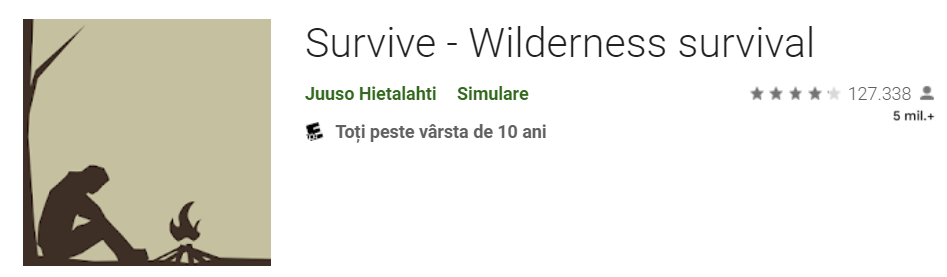
\includegraphics[width=15cm, height=5cm]{Images/OriginalBanner.png}}
		\end{figure}
		\par \textbf{Juuso Hietalathi}\cite{Juuso} is a \textbf{game developer} from \textbf{Finnland}. He started working on the project during a \underline{24} hour \textbf{Game Design Contest}, where he \textbf{won first place} for his \textbf{idea} and \textbf{rough implementation}. It was so successful that he \textbf{continued development} with the intention of \textbf{selling} it. Many years later, the \textbf{game}(\textit{Fig.(b)}) has \textbf{millions of downloads} and there is an \textbf{Android} and \textbf{iOS remake} in the works.
		\begin{figure}[H]
			\centering
			\subfigure[\textbf{App Store Game Cover}]{\label{fig:b}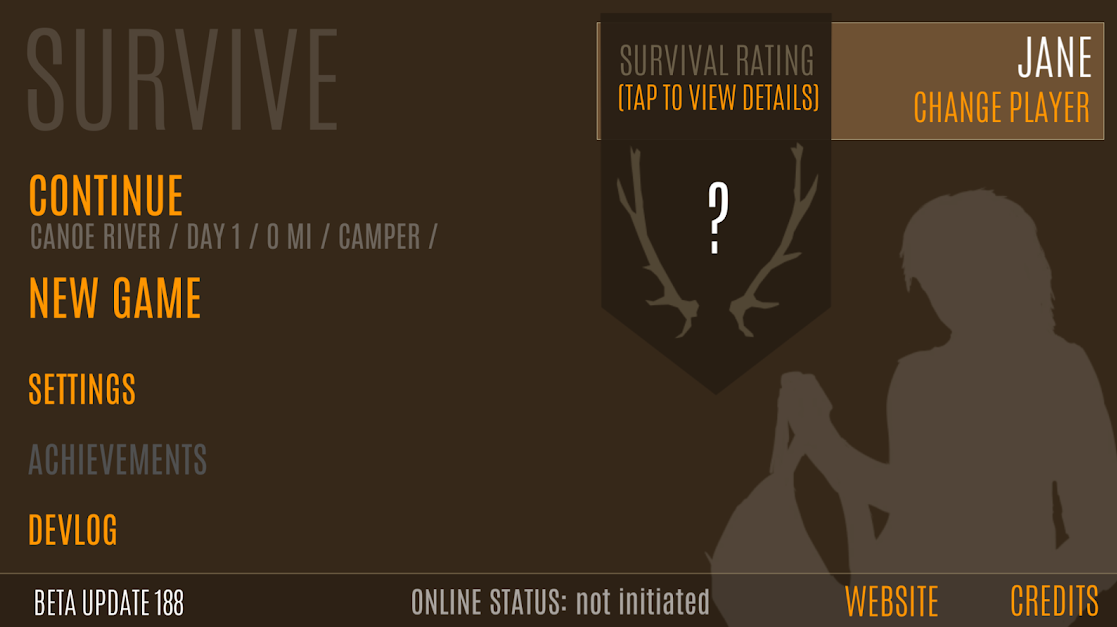
\includegraphics[width=10cm, height=5cm]{Images/OriginalCover.png}}
		\end{figure}
\newpage


\chapter*{Contribution}
\addcontentsline{toc}{chapter}{Contribution}
	\par The \textbf{thought process} leading to my \textbf{choice of project} contained many questions and requirements. It had to be a \textbf{game} in my favourite genres, \textbf{reasonable to implement} in one \textbf{semester} and full of \textbf{learning} potential.
	\par My decision, \textbf{"Survive - Wilderness survival"} turned out to have many \textbf{positives}. Almost \textbf{everything} is \textbf{new to me} in terms of implementation: the \textbf{platform}, the \textbf{genres}, the \textbf{gameplay}. I have never made an \textbf{Android Application} before, so I got to \textbf{experiment} with many new routes of \textbf{game} design and development. It was very \textbf{versatile} in terms of \textbf{languages} and \textbf{game engines}, so I could choose to be as \textbf{comfortable} or as \textbf{challenged} as I wanted to be.
	\par This \textbf{game} is \textbf{not new} to me. I \textbf{played} it before, it's the simplest \textbf{survival game} I have ever enjoyed. I had \textbf{tester insight}, I got to be the \textbf{target audience} for the project I was implementing. My \textbf{contribution} to the concept can be found in all the \textbf{differences} between the \textbf{original} and \textbf{my} development \textbf{journeys}. 

	\section*{Time Frame}
	\addcontentsline{toc}{section}{Time Frame}
		\par I did not spend \textbf{two years} designing a game from \textbf{scratch}, I spent \textbf{three months} \textbf{guessing} the steps someone else made, \textbf{analysing} why they made them and why they \textbf{succeeded}. I had a lot \textbf{less time} to complete a different set o \textbf{tasks}.

	\section*{Design Stages}
	\addcontentsline{toc}{section}{Design Stages}
		\par My \textbf{design decisions} were made as a result of a \textbf{two-step process}. \textbf{Replaying} the original game as many times as possible in order to \textbf{gather data} and guess what values were originally used, and \textbf{comparing} it to what I could or what I would rather \textbf{prefer} doing. 

	\section*{Technologies}
	\addcontentsline{toc}{section}{Technologies}
		\par The \textbf{original game} is implemented in \textbf{Unity}(a game engine) with \textbf{C\#}. I used \textbf{Python} and a \textbf{library}, leaving me a lot of \textbf{GUI elements} to make from \textbf{scratch}. This helped me a lot in my goal to \textbf{learn} as much as possible about the \textbf{basics}. \\ \\


	\par The \textbf{original} developer \textbf{designed} a game from \textbf{scratch}, with an \textbf{engine} that allowed a lot of freedom and \textbf{readily} implemented code, in the span of \textbf{2 years}. I took the role of \textbf{data analyst, tester, target audience} and \textbf{core back-end programmer} for \textbf{three months}, in a \textbf{different language}.

\newpage




\chapter{Game Design} 
	\section{Methodology}
		\par My \textbf{approach} resembled \textbf{Iterative Game Designing} the most. \textbf{Trying new things, testing, discarding} and \textbf{completely changing directions} was the only way I could \textbf{advance} towards my \textbf{main goal}, as I was implementing an \textbf{already existing game} just by \textbf{guessing} how it works.
		\par I used a \textbf{different language} and \textbf{no engine}. The first 3 weeks of the \textbf{development} were centered around \textbf{PyGame}, a cross-platform collection of modules for User Interfaces. I chose it because I had \textbf{experience} with it and I was \textbf{comfortable}. Unfortunately, it was \textbf{not suited} for \textbf{Android} applications, so I had to \textbf{discard everything} and \textbf{start from scratch} with \textbf{Kivy}, a framework I had never used before.
	      \par I was constantly trying to juggle the \textbf{back-end} and \textbf{front-end} integration, I couldn't tell how many \textbf{iterations} I would need and I had no way of \textbf{predicting} many problems in \textbf{advance}. 
		\par I believe that this \textbf{methodology} made me aware of what I don't know. I didn't stick to a topic's \textbf{specifics} and I didn't force myself to stop and \textbf{plan ahead} too much. It was \textbf{less rigid} and \textbf{more freeing} and \textbf{experimental}.
		\par As a result, I am much more \textbf{aware} of what \textbf{technologies exist} and how they \textbf{intertwine} to \textbf{solve a problem}, even if I don't know how they \textbf{work}. It taught me what my \textbf{minuses} are, what \textbf{kind of problems} exist and \textbf{where to look} for answers.  \\

		\begin{figure}[H]
			\centering
			\subfigure[\textbf{Iterative Game Design}]{\label{fig:a}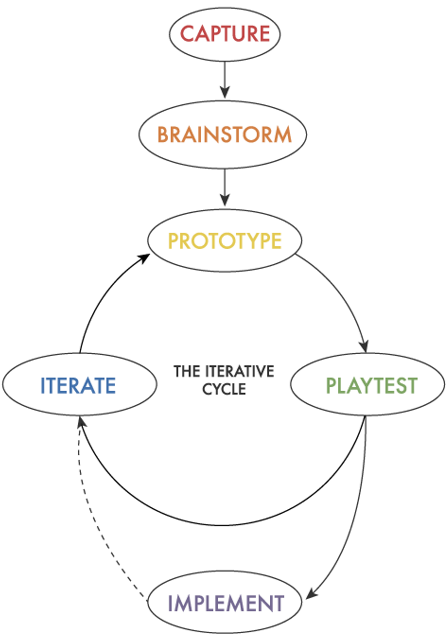
\includegraphics[width=5cm, height=8cm]{Images/IterativeGameDesign.png}}
		\end{figure}
	\section{User Interface}
		The \textbf{design} of the \textbf{User Interface} is meant to \textbf{resemble the original} one in terms of \textbf{screen layout}, but the \textbf{design} and \textbf{some button placements} were changed to suit my \textbf{preferences} and the \textbf{resources available}.

		\subsection{Screen Navigation Architecture}
			The \textbf{player} should be able to have the \textbf{same screen navigation experience} as it would with the \textbf{original game}. 
		\begin{figure}[H]
			\centering
			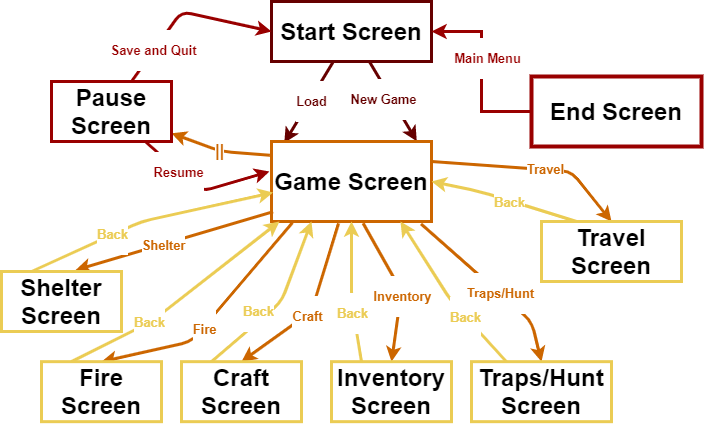
\includegraphics[width=15cm, height=20cm, keepaspectratio]{Images/ScreenArchitecture.png}\\
			\caption{\textbf{Screen Navigation}}
		\end{figure}

		\subsection{Screens}
			\par The entire \textbf{game} can be played with a simple \textbf{screen press}, \textbf{no scrolling} needed(including the inventory). There are \textbf{Pop Up} screens with \textbf{instructions} and \textbf{explanations} when necessary.
			\subsubsection{Main Menu and Pause Screens}
				\begin{figure}[H]
					\centering
					\subfigure[\textbf{Main Menu Screen}]{\label{fig:a}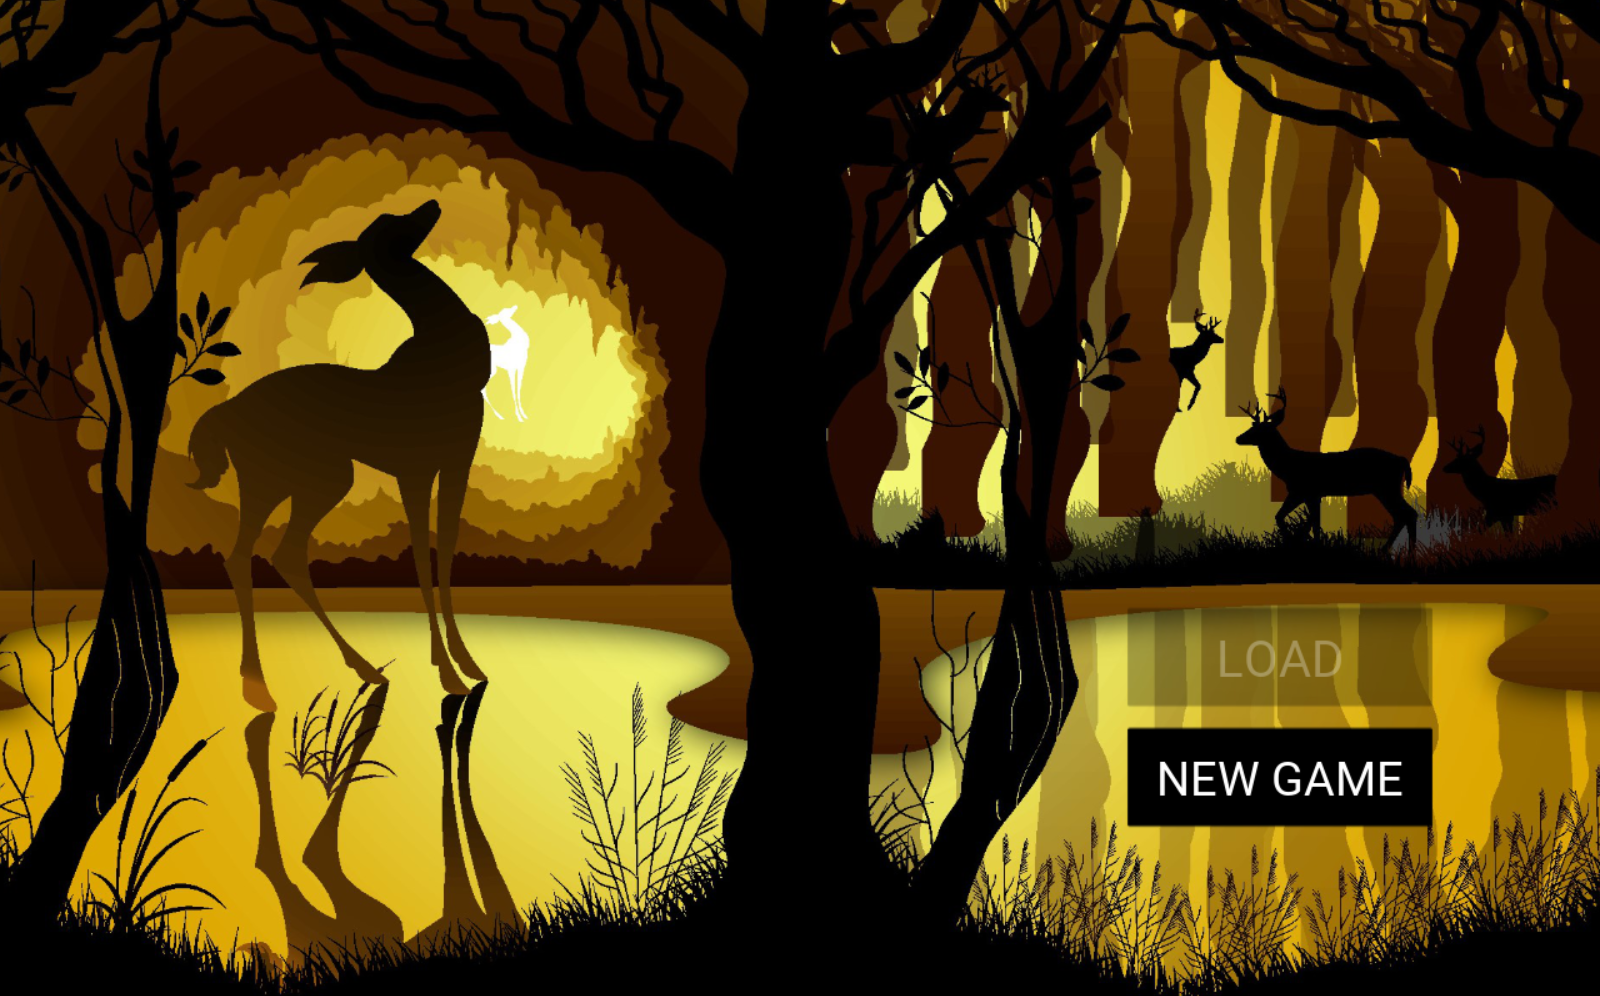
\includegraphics[width=7.5cm, height=4cm]{Images/MainMenu.png}}
				       \subfigure[\textbf{Pause Screen}]{\label{fig:b}
\includegraphics[width=7.5cm, height=4cm]{Images/Pause.png}}
				\end{figure}

			\subsubsection{Game Menu Screen}
				\begin{figure}[H]
					\centering
					\subfigure[\textbf{Game Menu Screen}]{\label{fig:c}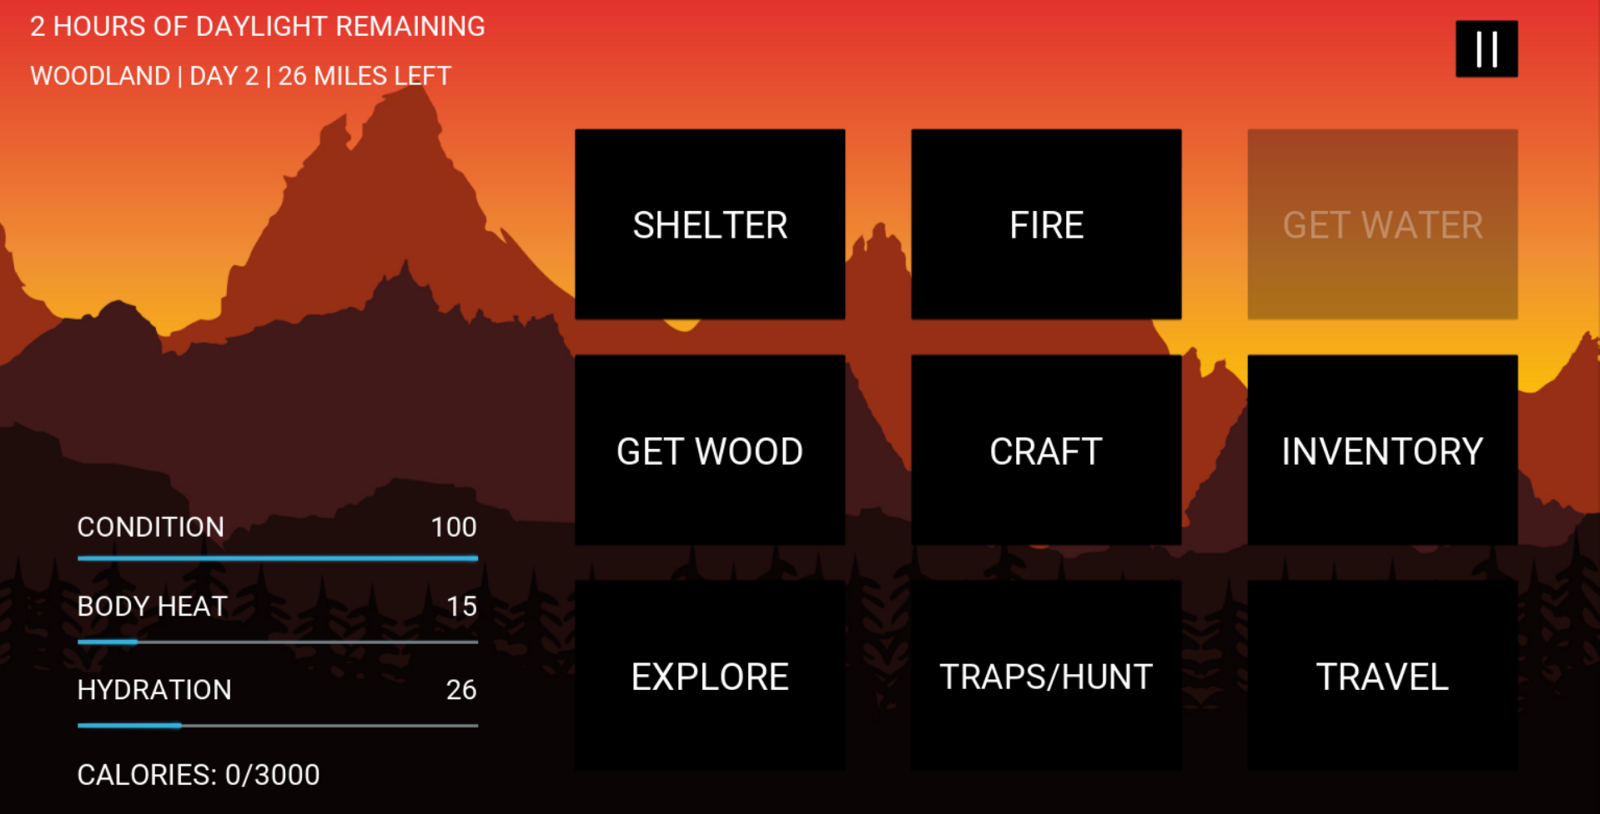
\includegraphics[width=15cm, height=8cm]{Images/Game.png}}
				\end{figure}

			\subsubsection{Crafting Menu Screen}
				\begin{figure}[H]
					\centering
					\subfigure[\textbf{Crafting Menu Screen 1}]{\label{fig:d}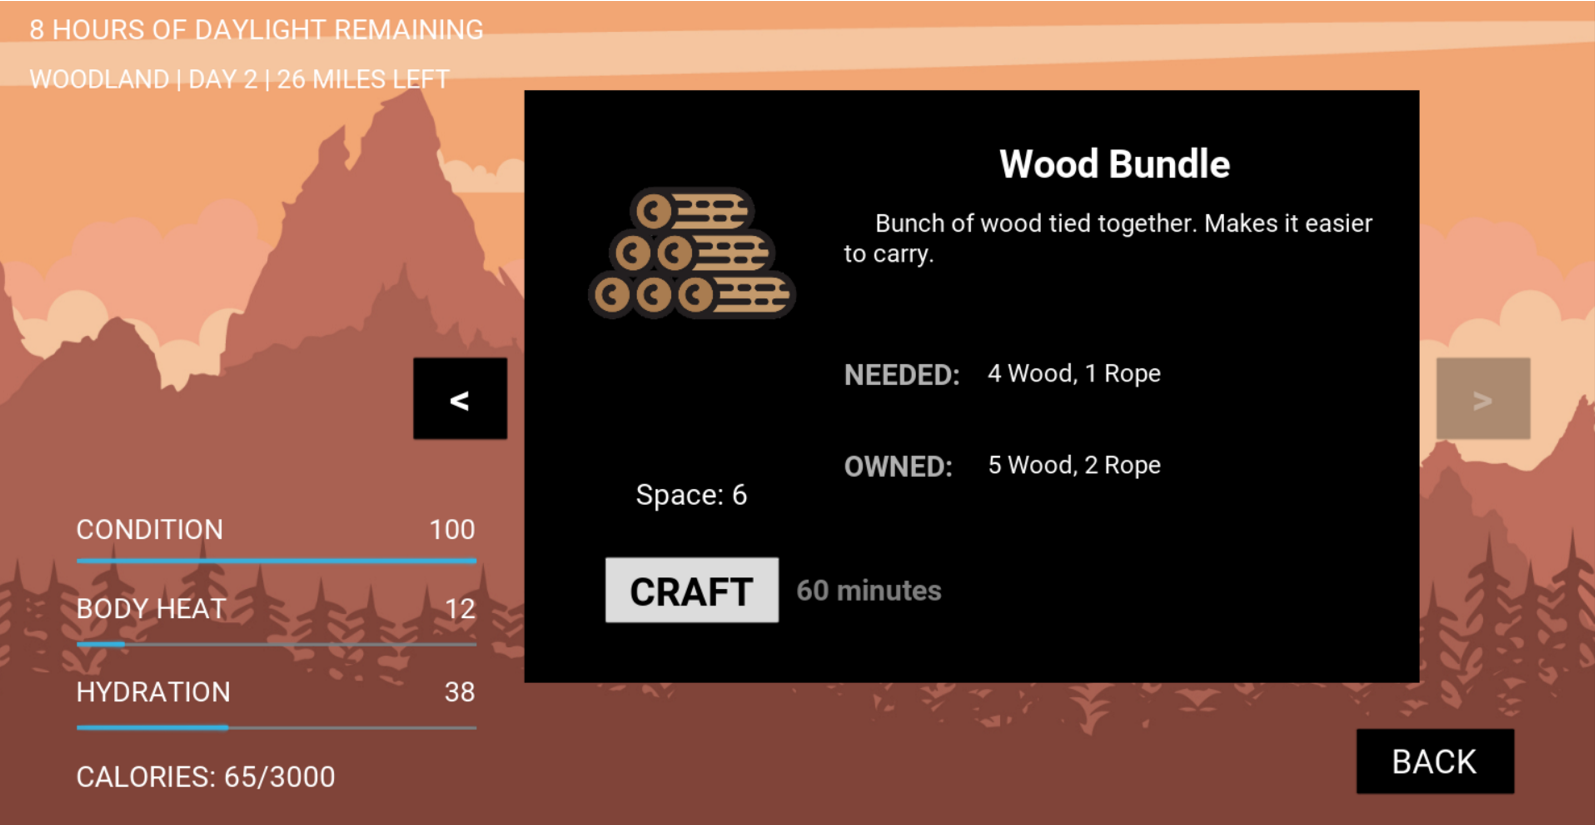
\includegraphics[width=7.5cm, height=4cm]{Images/Craft1.png}}
				       \subfigure[\textbf{Crafting Menu Screen 2}]{\label{fig:e}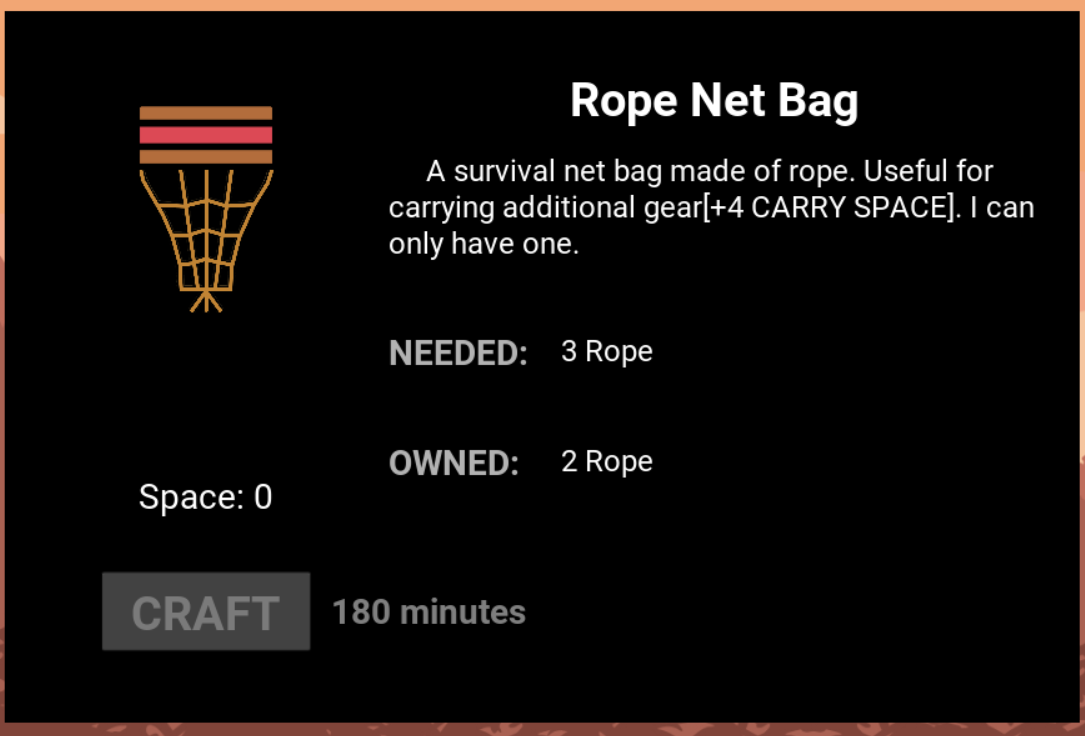
\includegraphics[width=7.5cm, height=4cm]{Images/Craft2.png}}
				\end{figure}

			\subsubsection{Shelter and Traps Screens}
				\begin{figure}[H]
					\centering
					\subfigure[\textbf{Shelter Screen}]{\label{fig:f}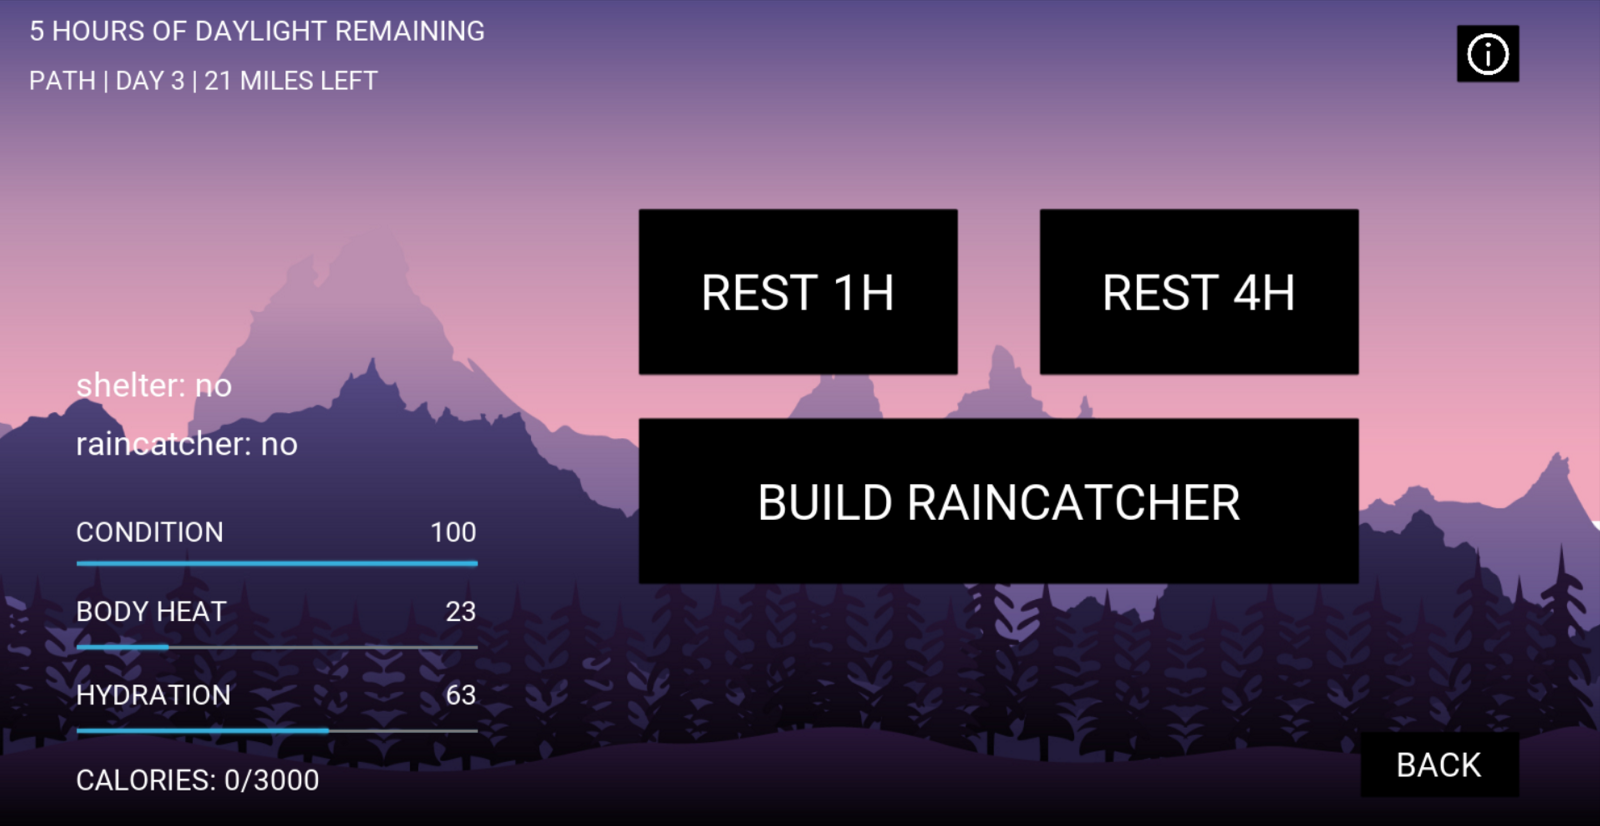
\includegraphics[width=7.5cm, height=3.8cm]{Images/Shelter.png}}
				       \subfigure[\textbf{Traps Screen}]{\label{fig:g}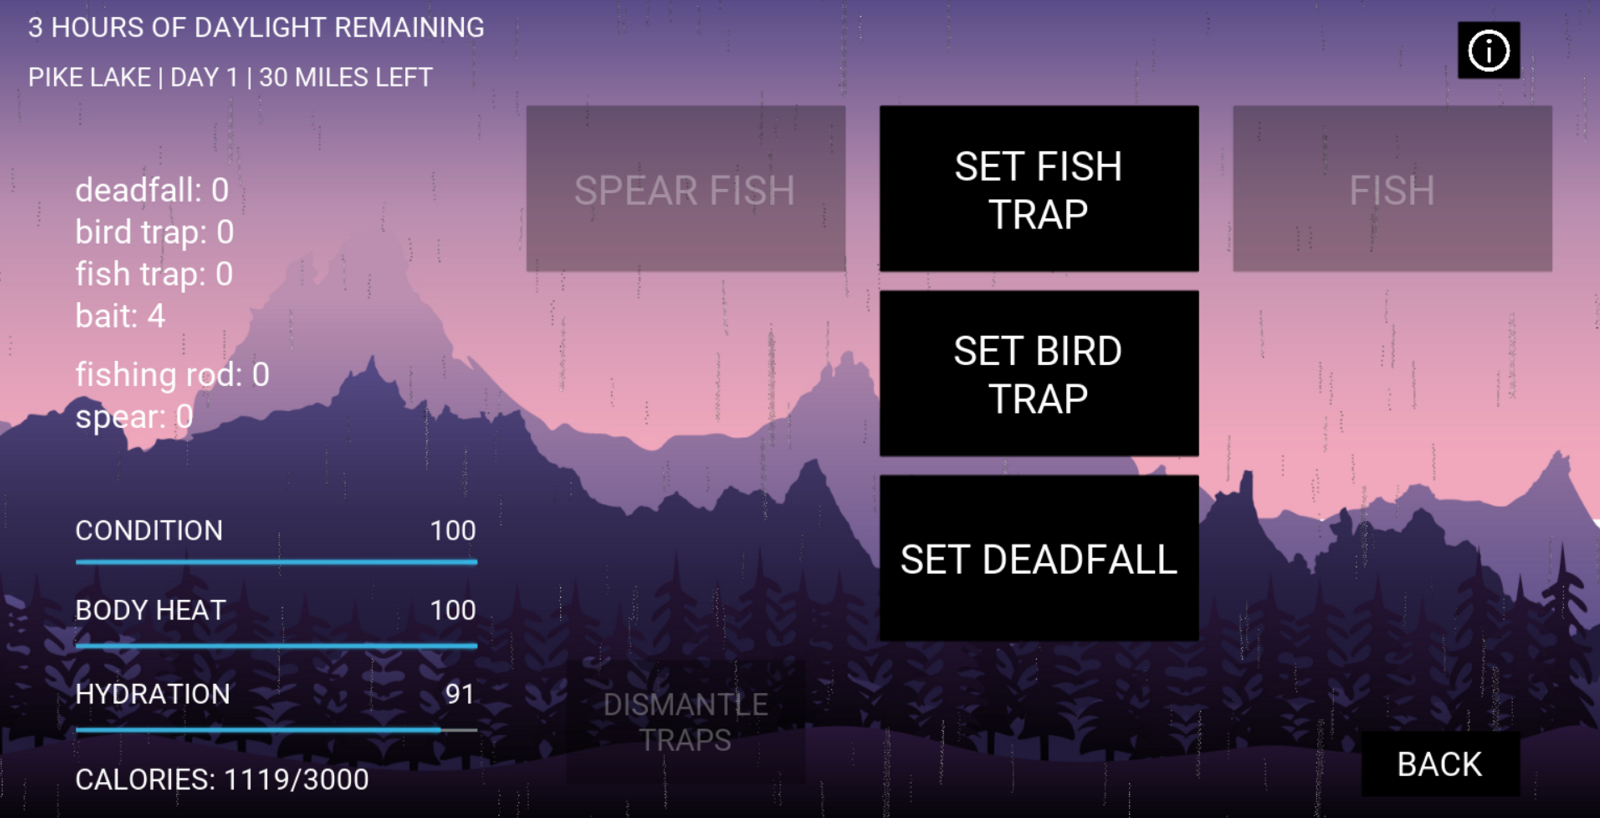
\includegraphics[width=7.5cm, height=3.8cm]{Images/Traps.png}}
				\end{figure}
			\subsubsection{Inventory Screen}
				\begin{figure}[H]
					\centering
					\subfigure[\textbf{Inventory Screen 1}]{\label{fig:j}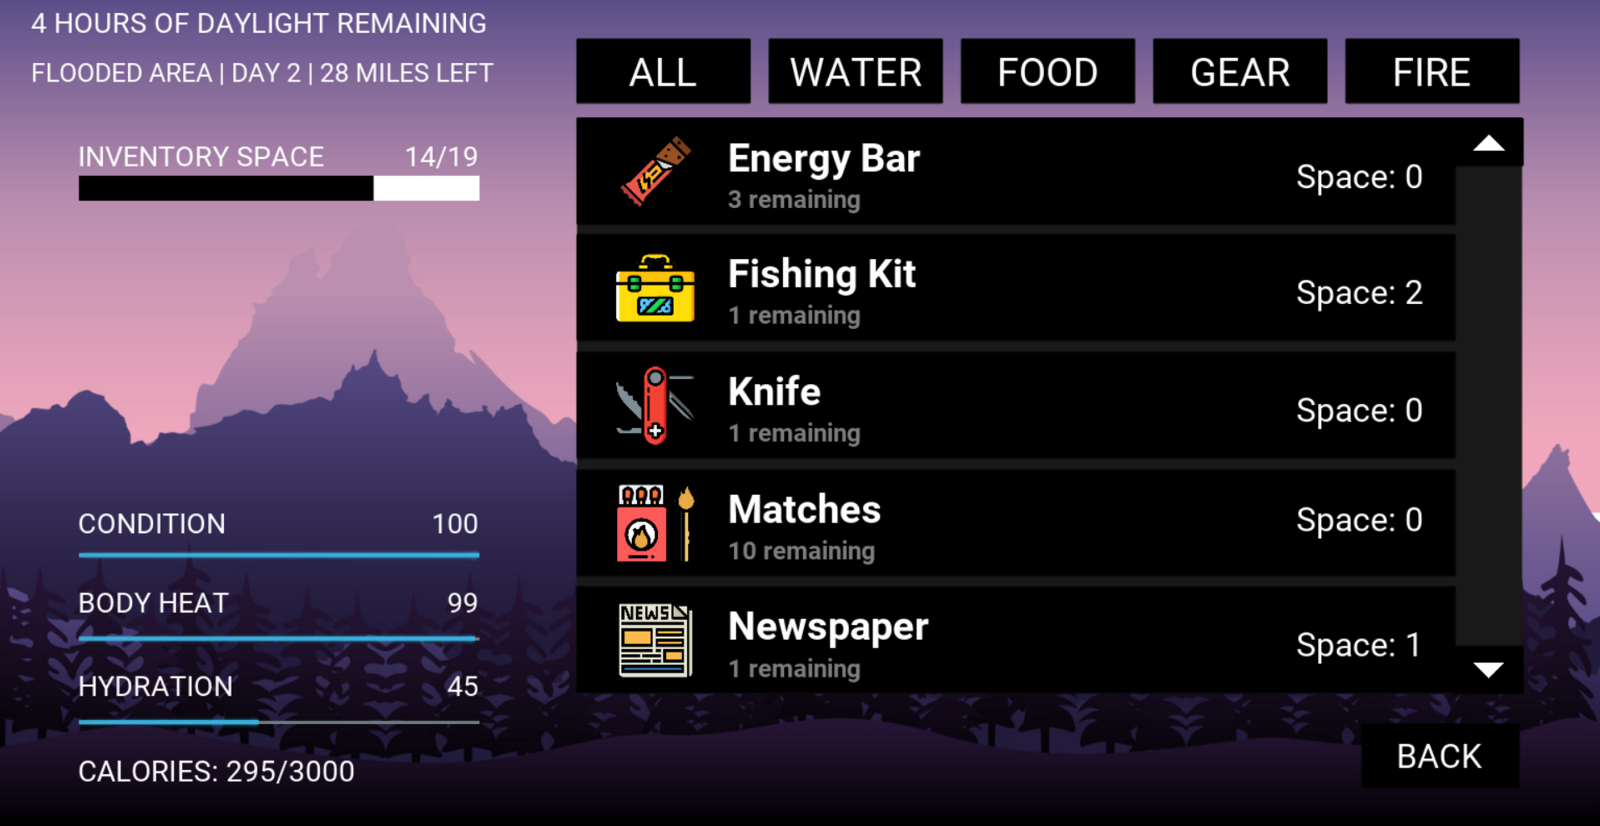
\includegraphics[width=7.5cm, height=3.8cm]{Images/Inventory3.png}}
					\subfigure[\textbf{Inventory Screen 2}]{\label{fig:h}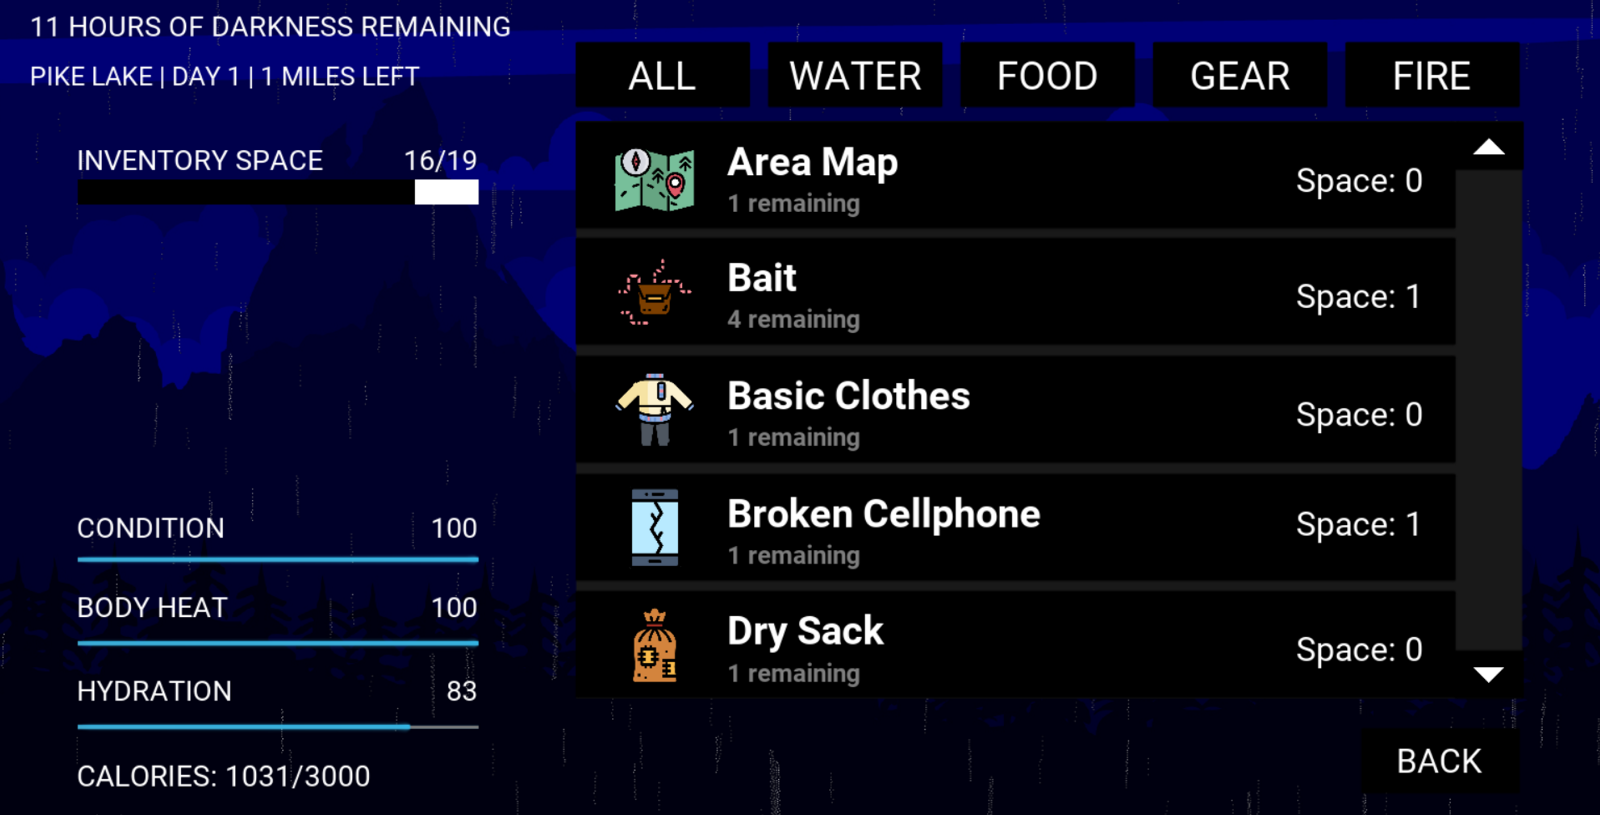
\includegraphics[width=7.5cm, height=3.8cm]{Images/Inventory1.png}}
				\end{figure}
			\subsubsection{Fire Screen}
				\begin{figure}[H]
					\centering
					\subfigure[\textbf{Fire Screen 1}]{\label{fig:l}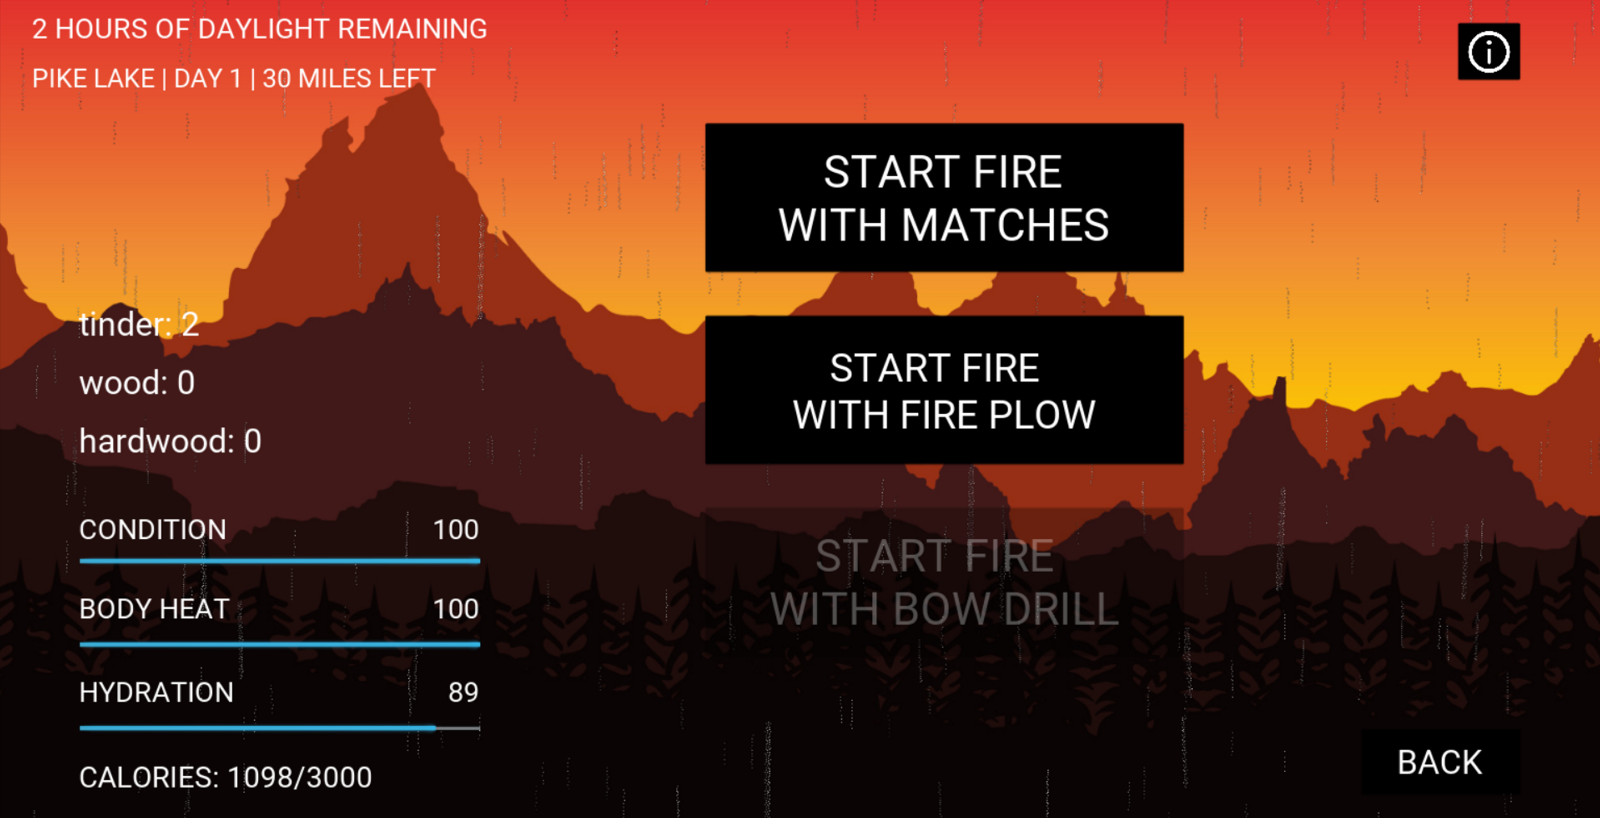
\includegraphics[width=7.5cm, height=3.8cm]{Images/Fire1.png}}
				       \subfigure[\textbf{Fire Screen 2}]{\label{fig:m}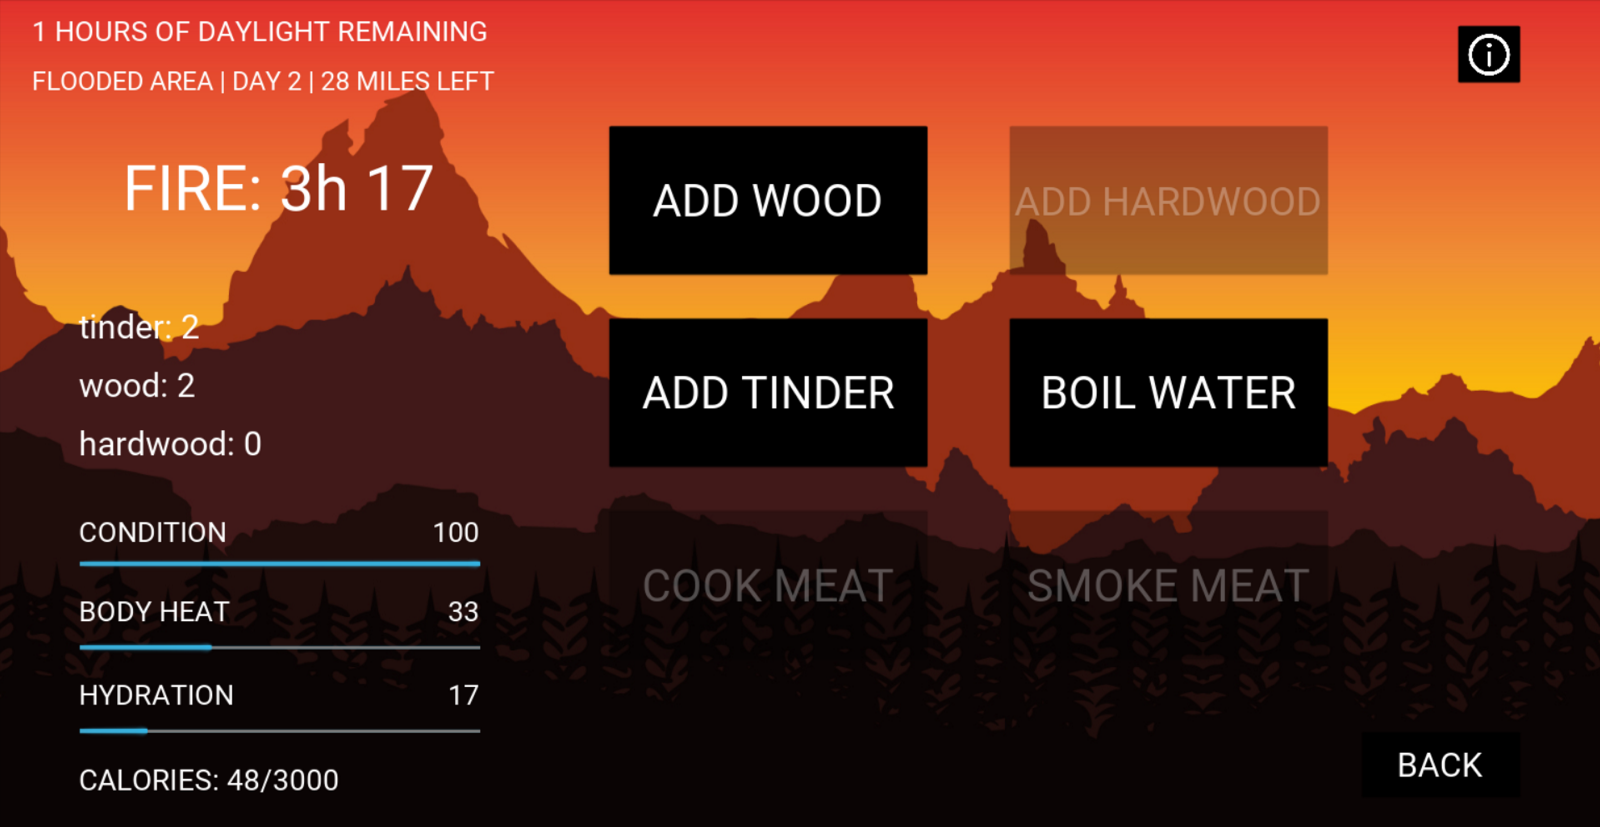
\includegraphics[width=7.5cm, height=3.8cm]{Images/Fire2.png}}
				\end{figure}
			\subsubsection{Travel Screen}
				\begin{figure}[H]
					\centering
					\subfigure[\textbf{Travel Screen}]{\label{fig:n}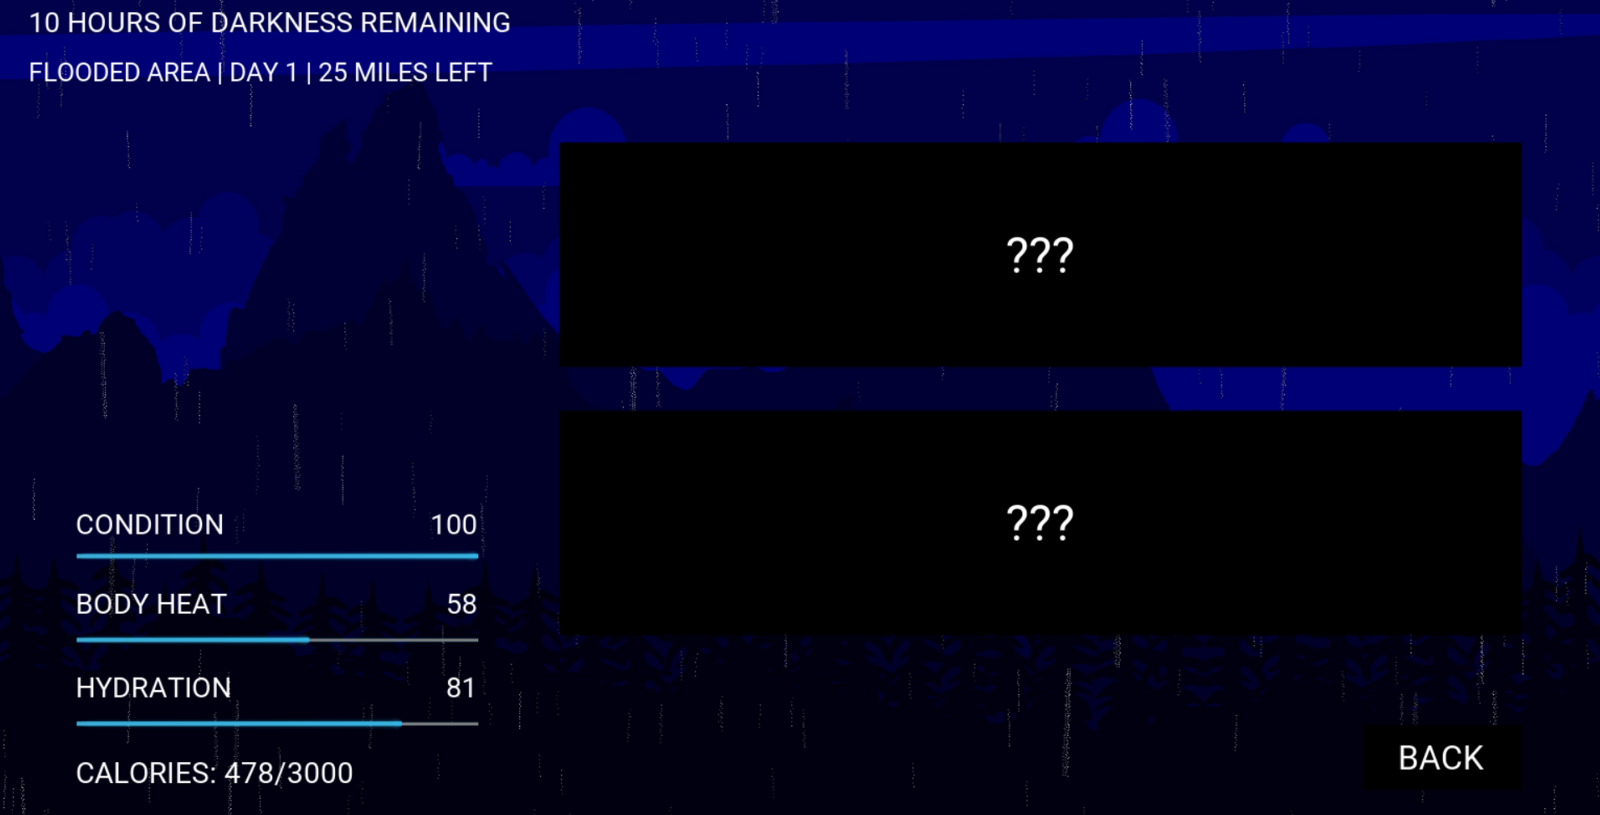
\includegraphics[width=7.5cm, height=3.8cm]{Images/Travel1.png}}
				       \subfigure[\textbf{Travel Screen with Flashlight}]{\label{fig:o}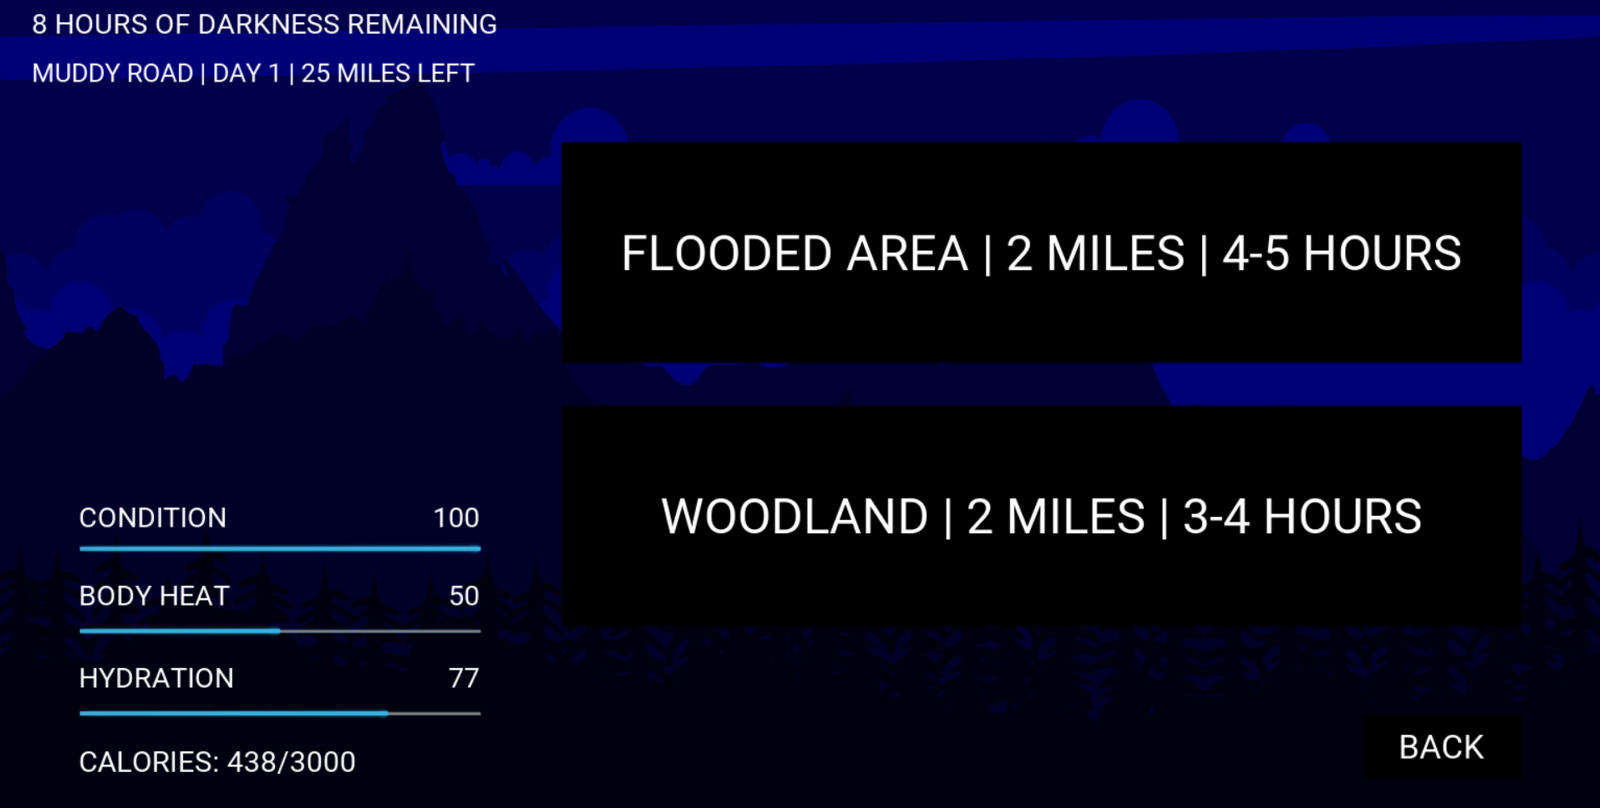
\includegraphics[width=7.5cm, height=3.8cm]{Images/Travel2.png}}
				\end{figure}

			\subsubsection{End Screen}
				\begin{figure}[H]
					\centering
					\subfigure[\textbf{Win Screen}]{\label{fig:p}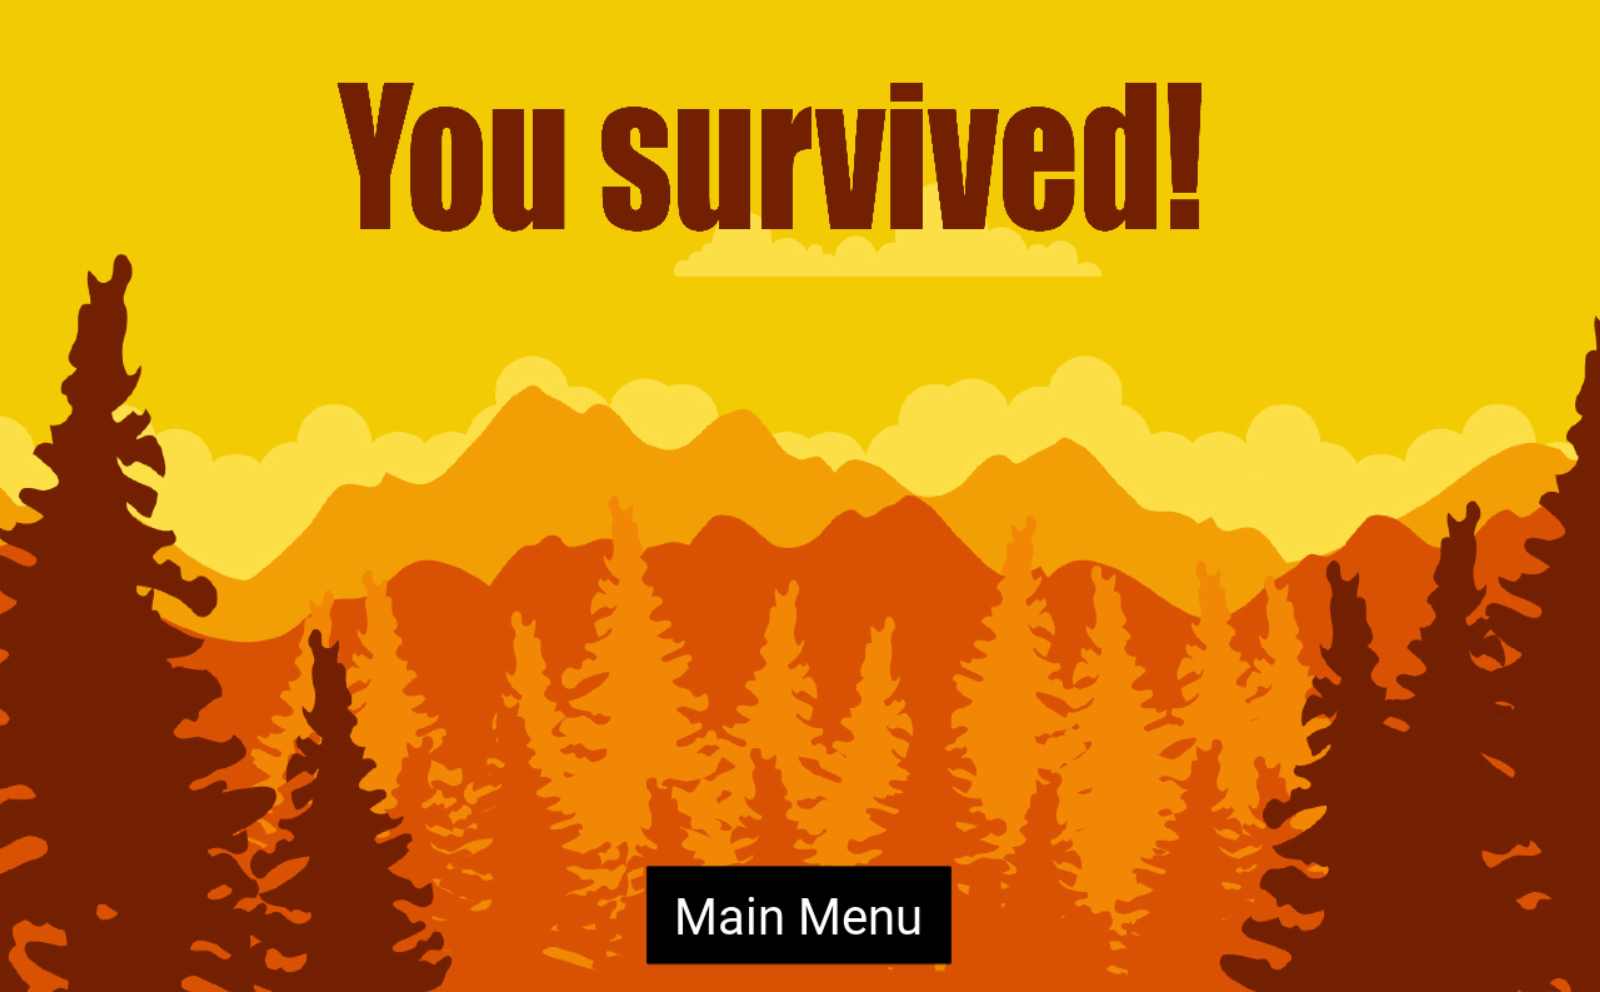
\includegraphics[width=7.5cm, height=4cm]{Images/Win.png}}
				       \subfigure[\textbf{Loss Screen}]{\label{fig:q}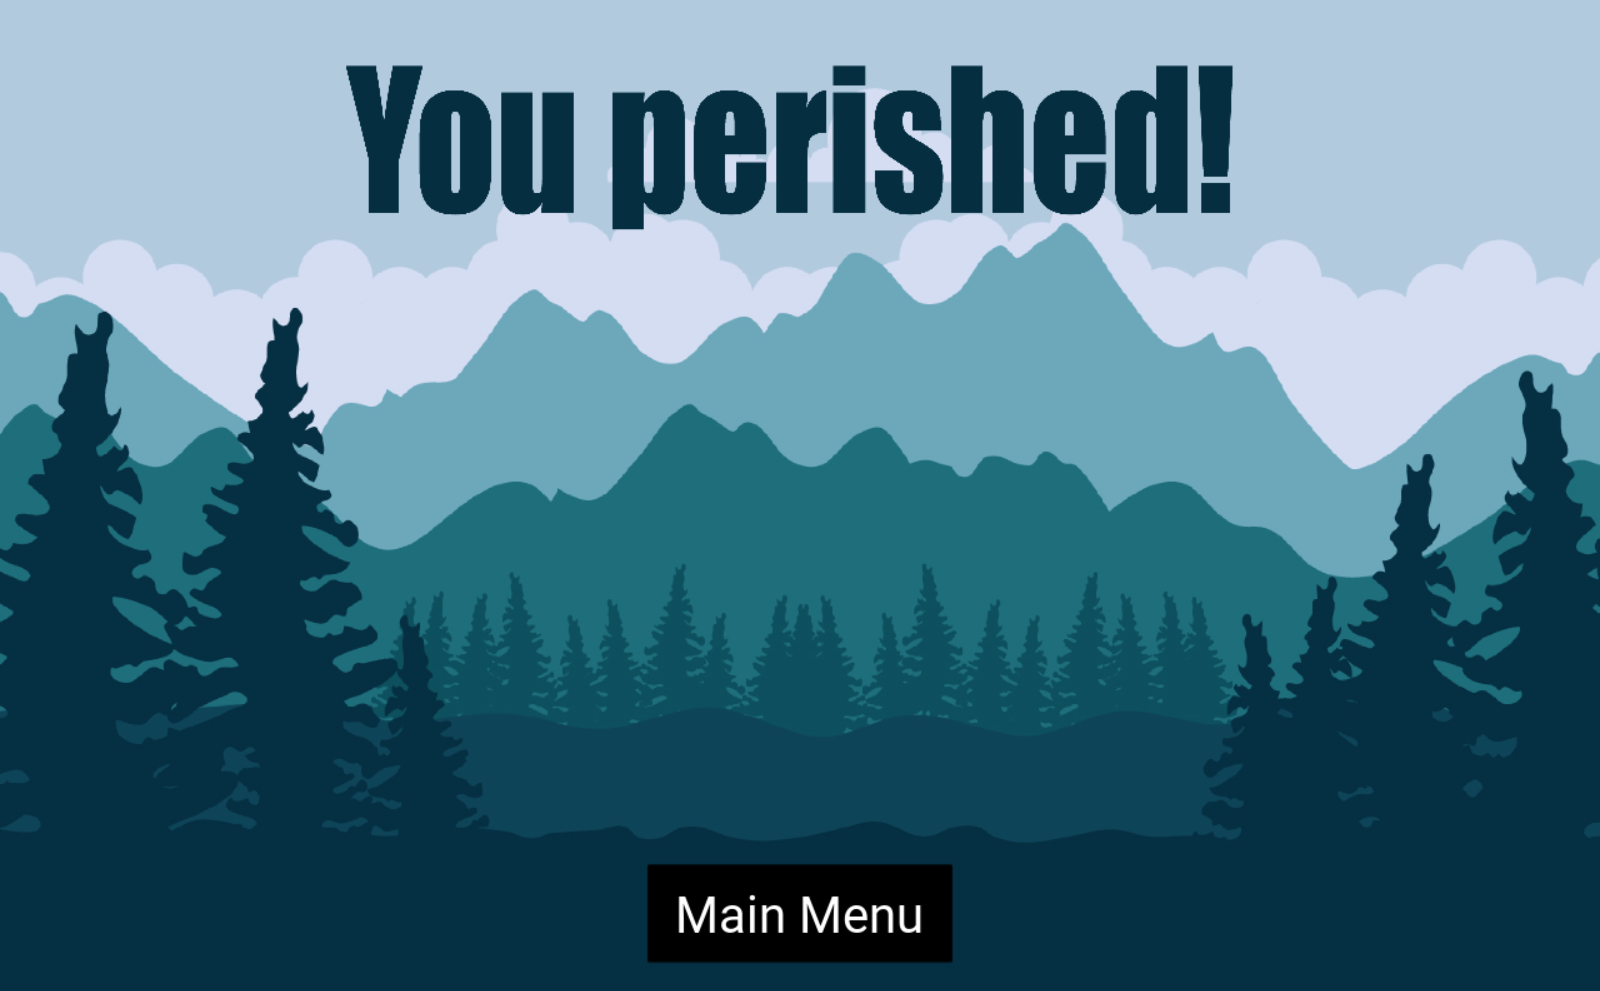
\includegraphics[width=7.5cm, height=4cm]{Images/Loss.png}}
				\end{figure}

\newpage




\chapter{Gameplay} 

	\section{Objective}
		\par The main goal is \textbf{SURVIVING}: away from the \textbf{forest} and back to \textbf{civilization}.
		
		\subsection{Environment}
			\par The \textbf{player} starts the game and immediately gets bombarded with \textbf{information} about its surroundings. At the \textbf{Pike Lake}, in the \textbf{middle of the woods}, \textbf{early afternoon}, during \textbf{heavy rain} that has covered the car tire tracks...with no easy way out in sight. It has no choice but to find a way to \textbf{survive}. 
			\par The \textbf{time, day, location, status bars, weather} and \textbf{remaining miles} to safety are visible on the \textbf{main screen}, ready for strategy planning.
			
		\subsection{Time}
			\par The \textbf{game time} is \underline{one hour} for every \underline{3 real minutes}. Instant actions such as \textbf{sleeping, travelling, crafting} and \textbf{exploring} take \underline{2 seconds} for any specified amount of time required for them. 
			\par The game is designed to offer the player enough time to \textbf{think, strategise} or \textbf{peruse} the inventory while taking no time in \textbf{advancing} the \textbf{story line}. Just like chess, an advanced \textbf{"speedrun"} can be completed in \underline{5 minutes}, while a \textbf{thought-out}(but poorly played) round can take up \underline{one hour and a half} with no bore or frustration from the player.
		
		\subsection{Weather}
				\par At the beginning, the \textbf{main character} is secluded by \textbf{rain}. The screen displays a ".gif" raindrop file and any action away from the car can swiftly lead to an \textbf{abrupt ending}. The car acts as a \textbf{shelter} that allows the game to still \textbf{start strong} and create the sense of urgency in order to set the \textbf{mechanics, objectives} and \textbf{priorities} for the player. 
			\par The lake is the \textbf{only} location that completely removes the \textbf{body heat depletion}. After leaving the lake,\textbf{ rain} will be the worst enemy against avoiding hypothermia and death. The user will learn that \textbf{sleeping} with surrounding warmth and \textbf{preparing for travelling} the next day is the best way to spend the night. Another tutorial-like benefit is showcasing that \textbf{clean, safe water} can be collected using a \textbf{raincatcher}, while the locations' existing sources are \textbf{dirty}.
			\par The \textbf{weather} also acts as an incentive to \textbf{explore} the very first day, which serves many purposes: teaching the \textbf{mechanic}, showing that \textbf{resources} are \textbf{not limited}, exemplifying the \textbf{status bar loss} during actions and making the player realize that Pike Lake \textbf{resources} are exclusive to it and extremely \textbf{important} to have for the rest of the \textbf{gameplay}. A \textbf{raining session} is anywhere between \underline{8} and \underline{72 hours}. The \textbf{cool down} is \underline{5} to \underline{24 hours}.
		
		\subsection{Day Time}
			\par The best time to \textbf{travel} and execute any \textbf{action} away from the current base is while it's \textbf{sunny}. There are \textbf{24 hours} in a game day, \underline{12} of daylight of \underline{12} with darkness.
			\par The player \textbf{can't see} the next possible \textbf{travel locations} without a \textbf{flashlight}. Trying to \textbf{explore, collect wood} and \textbf{set traps} will mainly result in \textbf{failure}. A flashlight can only be obtained while exploring at the Pike Lake. The item can \textbf{never} be found again after that and may even \textbf{break}.
			\par \textbf{Heat} depletes rapidly at \textbf{night}, especially during \textbf{rain}, a combination that will mostly result in game \textbf{loss}. The best night strategies are keeping a \textbf{lit fire, sleeping, crafting,} using \textbf{inventory items} and \textbf{planning to take off} first thing in the morning. 
		
		\subsection{Shelter}
			\par There is \textbf{warmth} from the \textbf{car} at the beginning of the game. Future locations require \textbf{fire} to at least stop the \textbf{heat} from dropping, which is next to that area's \textbf{place of rest} and \textbf{settlement}, also known as the \textbf{shelter}.
			\par The player may \textbf{sleep} the nights away or \textbf{build a raincatcher} from a \textbf{trash bag} in order collect \textbf{clean water}.

		\subsection{Locations}
			\par The \textbf{initial location} of the player is at \textbf{Pike Lake}. If it travels, it can \textbf{never return} again, as it is headed to the main \textbf{road}, in the opposite direction. 
			\par There are \underline{5} other \textbf{location types}(\textit{Table 2.1}) that serve as an \textbf{environment template}. The \textbf{player} may encounter the same kind of area \textbf{multiple times}, each with different faults and benefits. One may offer \textbf{water, certain resources} and \textbf{animals}, while the \textbf{road} to another could be \textbf{walked faster}.
			\begin{longtable}{|C{7em}|C{4.3em}|C{4.3em}|C{4.3em}|C{4.3em}|C{3.7em}|C{5em}|}
			   \toprule
			   \rowcolor[rgb]{ .647,  .647,  .647} \textcolor[rgb]{ 1,  1,  1}{\textbf{Locations}} & \cellcolor[rgb]{ .859,  .859,  .859}\textbf{Pike Lake} & \cellcolor[rgb]{ .859,  .859,  .859}\textbf{Flooded Area} & \cellcolor[rgb]{ .859,  .859,  .859}\textbf{Muddy Road} & \cellcolor[rgb]{ .859,  .859,  .859}\textbf{Muddy Area} & \cellcolor[rgb]{ .859,  .859,  .859}\textbf{Path} & \cellcolor[rgb]{ .859,  .859,  .859}\textbf{Woodland} \\
			   \bottomrule	
			\caption{\textbf{Game Locations}}
			\end{longtable}		
		

	\section{Status Bars}
		
		\par There are \underline{4} \textbf{values} to keep an eye on: \textbf{Condition, Body Heat, Hydration} and \textbf{Calories}. All of them can go \textbf{below} \underline{0}, signifying that the player is on its last breath. \textbf{Calories} do not lead to \textbf{death}, as a person can \textbf{realistically} go weeks \textbf{without food}, but the \textbf{game ends} when any of the others reach -\underline{15\%}.  
		
		\subsection{Condition}
			\par \textbf{Condition} is a value that can be mostly \textbf{left alone}. It improves \textbf{slightly} during the day if it's not maxed out already.  Its main purpose arises in times of desperation.
			\par The \textbf{player} may find itself in a \textbf{dire situation}, with only \textbf{dirty water}, \textbf{nearing death thirst} and \textbf{no way} to swiftly \textbf{start a fire}. Drinking it would offer a way out \textbf{once or twice}(\textit{Table 2.2}), but more is mainly \textbf{luck}. \textbf{Spoiled meat} could offer the necessary \textbf{calories} to travel the \textbf{last miles} fast as to not die of thirst, \textbf{raw meat} could be near \textbf{expiring}.
			\par There is a slight \textbf{timely increase}, as well as \textbf{bandages} to fix \textbf{travel} and \textbf{hypothermia} \textbf{wounds}, but \textbf{Condition} is mostly an end game \textbf{gamble}.

			\begin{longtable}{|C{6em}|C{6em}|C{6em}|C{6em}|C{9em}|}
			   \toprule
			   \rowcolor[rgb]{ .647,  .647,  .647} \textcolor[rgb]{ 1,  1,  1}{\textbf{Item}} & \cellcolor[rgb]{ .859,  .859,  .859}\textbf{Bandages} & \cellcolor[rgb]{ .859,  .859,  .859}\textbf{Raw Meat} & \cellcolor[rgb]{ .859,  .859,  .859}\textbf{Spoiled Meat}  & \cellcolor[rgb]{ .859,  .859,  .859}\textbf{Unsafe Water Bottle}   \\
			    \midrule
			    \rowcolor[rgb]{ .647,  .647,  .647} \textcolor[rgb]{ 1,  1,  1}{\textbf{Condition}}  & \cellcolor[rgb]{ .929,  .929,  .929}\textbf{20} & \cellcolor[rgb]{ .929,  .929,  .929}\textbf{[-70, -30]} & \cellcolor[rgb]{ .929,  .929,  .929}\textbf{[-90, -50]} & \cellcolor[rgb]{ .929,  .929,  .929}\textbf{[-60, 0]} \\	
			    \bottomrule	
			\caption{\textbf{Values} of \textbf{Condition} Changing \textbf{Items}}
			\end{longtable}
		
		\subsection{Body Heat}
			\par There are \underline{5} factors that influence \textbf{heat depletion}: \textbf{Shelter}(S), \textbf{Rain}(R), \textbf{Day Time}(D), \textbf{Clothing}(C) and \textbf{Fire}(F). 
			\par If the current location is \textbf{Pike Lake}, the player only \textbf{loses heat} if it \textbf{explores} or \textbf{travels}. That is the \textbf{only} time \textbf{shelter} is available. It can be \textbf{raining}, it can be \textbf{day or night} and the \textbf{fire} can be \textbf{lit} or not. The player \textbf{starts off} with a set of \textbf{clothing}, but it can be torn for \textbf{pieces of cloth}.
			\par The \textbf{table} below(\textit{Table 2.3}) shows all the remaining \textbf{factor combinations} and the \textbf{values} they influence \textbf{Body Heat} with every \textbf{hour}. Each \underline{"N"} preceding a factor \textbf{letter}(mentioned above) signifies \textbf{"not"}, so \underline{"NS"} would be no shelter. The code \textbf{"NSRNDCF"} reads as "\textbf{no shelter, rain, no day}(night)\textbf{, clothing}(player has it)\textbf{, fire}(is lit)" and depletes \textbf{heat} by \underline{-3} for each \textbf{hour} that the game is in that state.
			

		\begin{longtable}{|C{8em}|C{8em}|C{8em}|C{8em}|}
			   \toprule
			    \rowcolor[rgb]{ .851,  .851,  .851} \textbf{NSRDCF} & \cellcolor[rgb]{ .929,  .929,  .929}\textbf{NSNRDCF} & \textbf{NSRNDCF} & \cellcolor[rgb]{ .929,  .929,  .929}\textbf{NSRDNCF} \\
			    \midrule
			    \rowcolor[rgb]{ .851,  .851,  .851} \textbf{-2} & \cellcolor[rgb]{ .929,  .929,  .929}\textbf{30} & \textbf{-3} & \cellcolor[rgb]{ .929,  .929,  .929}\textbf{-4,5} \\
			    \midrule
			    \rowcolor[rgb]{ .929,  .929,  .929} \textbf{NSRDCNF} & \cellcolor[rgb]{ .851,  .851,  .851}\textbf{NSNRNDCF} & \textbf{NSNRDNCF} & \cellcolor[rgb]{ .749,  .749,  .749}\textbf{NSNRDCNF} \\
			    \midrule
			    \rowcolor[rgb]{ .929,  .929,  .929} \textbf{-3,5} & \cellcolor[rgb]{ .851,  .851,  .851}\textbf{25} & \textbf{28} & \cellcolor[rgb]{ .749,  .749,  .749}\textbf{0,5} \\
			    \midrule
			    \rowcolor[rgb]{ .851,  .851,  .851} \textbf{NSRNDNCF} & \cellcolor[rgb]{ .929,  .929,  .929}\textbf{NSRNDCNF} & \textbf{NSRDNCNF} & \cellcolor[rgb]{ .929,  .929,  .929}\textbf{NSNRNDNCF} \\
			    \midrule
			    \rowcolor[rgb]{ .851,  .851,  .851} \textbf{-4,5} & \cellcolor[rgb]{ .929,  .929,  .929}\textbf{-8} & \textbf{-6} & \cellcolor[rgb]{ .929,  .929,  .929}\textbf{23} \\
			    \midrule
			    \rowcolor[rgb]{ .929,  .929,  .929} \textbf{NSNRNDCNF} & \cellcolor[rgb]{ .851,  .851,  .851}\textbf{NSNRDNCNF} & \textbf{NSRNDNCNF} & \cellcolor[rgb]{ .851,  .851,  .851}\textbf{NSNRNDNCNF} \\
			    \midrule
			    \rowcolor[rgb]{ .929,  .929,  .929} \textbf{-4,5} & \cellcolor[rgb]{ .851,  .851,  .851}\textbf{0} & \textbf{-9,5} & \cellcolor[rgb]{ .851,  .851,  .851}\textbf{-6} \\
			    \bottomrule
				\caption{Game \textbf{Hourly Heat Loss} Codes and Values}
		 \end{longtable}
		
		\subsection{Hydration}
			\par \textbf{Hydration} is the most \textbf{obvious} and \textbf{mediocre} status to look after. The player \textbf{starts} with several \textbf{bottles} of liquid and it can also collect more using \textbf{empty bottles} found at \textbf{Pike Lake}.
			\par \textbf{Building a raincatcher}, collecting from \textbf{water sources}(Pike Lake, Muddy Areas and Flooded Areas) and finding \textbf{edible berries}(\textit{Table 2.4}) exploring are the ways to \textbf{get water}.
			
			\begin{longtable}{|C{5em}|C{4em}|C{4em}|C{4em}|C{4em}|C{4em}|}
			   \toprule
			   \rowcolor[rgb]{ .647,  .647,  .647} \textcolor[rgb]{ 1,  1,  1}{\textbf{Item}} & \cellcolor[rgb]{ .859,  .859,  .859}\textbf{Safe Water Bottle} & \cellcolor[rgb]{ .859,  .859,  .859}\textbf{Unsafe Water Bottle} &\cellcolor[rgb]{ .859,  .859,  .859}\textbf{Squirrel Juice} &\cellcolor[rgb]{ .859,  .859,  .859}\textbf{Soda Bottle} & \cellcolor[rgb]{ .859,  .859,  .859}\textbf{Edible Berries}  \\
			    \midrule
			    \rowcolor[rgb]{ .647,  .647,  .647} \textcolor[rgb]{ 1,  1,  1}{\textbf{Hydration}}  & \cellcolor[rgb]{ .929,  .929,  .929}\textbf{25} & \cellcolor[rgb]{ .929,  .929,  .929}\textbf{25} & \cellcolor[rgb]{ .929,  .929,  .929}\textbf{25} & \cellcolor[rgb]{ .929,  .929,  .929}\textbf{25} & \cellcolor[rgb]{ .929,  .929,  .929}\textbf{5} \\	
			    \bottomrule	
			\caption{\textbf{Values} of \textbf{Hydtration} Changing \textbf{Items}}
			\end{longtable}

		\subsection{Calories}
			\par The player \textbf{can't die} from \textbf{calorie loss}, but they are needed for \textbf{travelling}, as going below \underline{400} adds \underline{2} \textbf{extra hours} to the \textbf{length} of the journey.
			\begin{longtable}{|C{4em}|C{4em}|C{4em}|C{4em}|C{4em}|C{4em}|C{4em}|}
			   \toprule
			   \rowcolor[rgb]{ .647,  .647,  .647} \textcolor[rgb]{ 1,  1,  1}{\textbf{Item}} & \cellcolor[rgb]{ .859,  .859,  .859}\textbf{Energy Bar} &\cellcolor[rgb]{ .859,  .859,  .859}\textbf{Crickets} &\cellcolor[rgb]{ .859,  .859,  .859}\textbf{Maggots} &\cellcolor[rgb]{ .859,  .859,  .859}\textbf{Soda Bottle} & \cellcolor[rgb]{ .859,  .859,  .859}\textbf{Edible Berries} & \cellcolor[rgb]{ .859,  .859,  .859}\textbf{Squirrel Juice}  \\
			    \midrule
			    \rowcolor[rgb]{ .647,  .647,  .647} \textcolor[rgb]{ 1,  1,  1}{\textbf{Calories}} & \cellcolor[rgb]{ .929,  .929,  .929}\textbf{150} & \cellcolor[rgb]{ .929,  .929,  .929}\textbf{100} & \cellcolor[rgb]{ .929,  .929,  .929}\textbf{50} & \cellcolor[rgb]{ .929,  .929,  .929}\textbf{300} & \cellcolor[rgb]{ .929,  .929,  .929}\textbf{100} & \cellcolor[rgb]{ .929,  .929,  .929}\textbf{100}  \\	
			    \bottomrule	
			\caption{A. \textbf{Values} of \textbf{Calorie} Changing \textbf{Items}}
			\end{longtable}

			\begin{longtable}{|C{4em}|C{4em}|C{4em}|C{4em}|C{4em}|C{4em}|C{4em}|}
			   \toprule
			   \rowcolor[rgb]{ .647,  .647,  .647} \textcolor[rgb]{ 1,  1,  1}{\textbf{Item}} & \cellcolor[rgb]{ .859,  .859,  .859}\textbf{Smoked Jerky} & \cellcolor[rgb]{ .859,  .859,  .859}\textbf{Can of Peas} &\cellcolor[rgb]{ .859,  .859,  .859}\textbf{Edible Plant Part} &\cellcolor[rgb]{ .859,  .859,  .859}\textbf{Raw Meat} & \cellcolor[rgb]{ .859,  .859,  .859}\textbf{Spoiled Meat} & \cellcolor[rgb]{ .859,  .859,  .859}\textbf{Cooked Meat} \\
			    \midrule
			    \rowcolor[rgb]{ .647,  .647,  .647} \textcolor[rgb]{ 1,  1,  1}{\textbf{Calories}}  & \cellcolor[rgb]{ .929,  .929,  .929}\textbf{300} & \cellcolor[rgb]{ .929,  .929,  .929}\textbf{300} & \cellcolor[rgb]{ .929,  .929,  .929}\textbf{50} & \cellcolor[rgb]{ .929,  .929,  .929}\textbf{400} & \cellcolor[rgb]{ .929,  .929,  .929}\textbf{200} & \cellcolor[rgb]{ .929,  .929,  .929}\textbf{800} \\	
			    \bottomrule		
			\caption{B. \textbf{Values} of \textbf{Calorie} Changing \textbf{Items}}
			\end{longtable}


	\section{Inventory}
		\par The \textbf{Inventory} has a \textbf{space}(not weight) \textbf{capacity} that be increased with \textbf{extra carry items} that are crafted or owned from the beggining.  If the \textbf{space limit} is \textbf{exceeded}, then the player \textbf{can't travel}.
		\par There are \textbf{interesting ways} of going around this, such as \textbf{throwing stuff out}(the cellphone is useless and take 1 space point), crafting \textbf{compact items} from more voluminous ones(Wood Bundles), crafting \textbf{carry items}(Rope Net Bag, Pouch) and keeping \textbf{destructibles} \textbf{intact} until the \textbf{resulting resources} are needed, as they usually take \textbf{more space}. 

		\subsection{Items}
			\par The \textbf{Inventory} holds all of the player's \textbf{items} and allows their \textbf{manipulation}(Eating, Drinking, Throwing Out, Destruction). 
			\par There are \underline{5} categories: \textbf{All}(A), \textbf{Gear}(G), \textbf{Fire}(Fi), \textbf{Food}(Fo) and \textbf{Water}(Wa) for \textbf{easy navigation}, as seen in Table 2.7.

			\begin{longtable}{|C{10.555em}|C{4.0em}|C{4.0em}|C{6.445em}|C{11.055em}|}
			    \toprule
			    \rowcolor[rgb]{ .647,  .647,  .647} \textcolor[rgb]{ 1,  1,  1}{\textbf{Item}} & \textcolor[rgb]{ 1,  1,  1}{\textbf{Space}} & \textcolor[rgb]{ 1,  1,  1}{\textbf{Throw }} & \textcolor[rgb]{ 1,  1,  1}{\textbf{Category}} & \textcolor[rgb]{ 1,  1,  1}{\textbf{Items Obtained From Destruction}} \\
			    \midrule
			    \rowcolor[rgb]{ .859,  .859,  .859} \textbf{Area Map} & \textbf{0.0} & \textbf{Yes} & \textbf{A, G, Fi} & \textbf{Tinder} \\
			    \midrule
			    \rowcolor[rgb]{ .929,  .929,  .929} \textbf{Backside Of A Paper} & \textbf{1.0} & \textbf{Yes} & \textbf{A, G} & \textbf{Tinder} \\
			    \midrule
			    \rowcolor[rgb]{ .859,  .859,  .859} \textbf{Bait} & \textbf{0.34} & \textbf{Yes} & \textbf{A, G} & \textbf{-} \\
			    \midrule
			    \rowcolor[rgb]{ .929,  .929,  .929} \textbf{Bandages} & \textbf{1.0} & \textbf{Yes} & \textbf{A, G} & \textbf{Tinder} \\
			    \midrule
			    \rowcolor[rgb]{ .859,  .859,  .859} \textbf{Basic Clothes} & \textbf{0.0} & \textbf{No} & \textbf{A, G} & \textbf{Piece of Cloth, Torn Clothes} \\
			    \midrule
			    \rowcolor[rgb]{ .929,  .929,  .929} \textbf{Birch Bark} & \textbf{1.0} & \textbf{Yes} & \textbf{A, Fi} & \textbf{Tinder} \\
			    \midrule
			    \rowcolor[rgb]{ .859,  .859,  .859} \textbf{Bow Drill} & \textbf{2.0} & \textbf{Yes} & \textbf{A, Fi} & \textbf{-} \\
			    \midrule
			    \rowcolor[rgb]{ .929,  .929,  .929} \textbf{Broken Cellphone} & \textbf{1.0} & \textbf{Yes} & \textbf{A, G} & \textbf{-} \\
			    \midrule
			    \rowcolor[rgb]{ .859,  .859,  .859} \textbf{Can of Peas} & \textbf{1.0} & \textbf{Yes} & \textbf{A, Fo} & \textbf{-} \\
			    \midrule
			    \rowcolor[rgb]{ .929,  .929,  .929} \textbf{Cattail Plant} & \textbf{1.0} & \textbf{Yes} & \textbf{A, Fo} & \textbf{Edible Plant Part, Plant Fiber, Tinder} \\
			    \midrule
			    \rowcolor[rgb]{ .859,  .859,  .859} \textbf{Cooked Meat} & \textbf{1.0} & \textbf{Yes} & \textbf{A, Fo} & \textbf{-} \\
			    \midrule
			    \rowcolor[rgb]{ .929,  .929,  .929} \textbf{Crickets} & \textbf{0.34} & \textbf{Yes} & \textbf{A, Fo} & \textbf{Bait} \\
			    \midrule
			    \rowcolor[rgb]{ .859,  .859,  .859} \textbf{Dead Bird} & \textbf{3.0} & \textbf{Yes} & \textbf{A, Fo} & \textbf{Raw Meat} \\
			    \midrule
			    \rowcolor[rgb]{ .929,  .929,  .929} \textbf{Dead Fish} & \textbf{1.0} & \textbf{Yes} & \textbf{A, Fo} & \textbf{Raw Meat} \\
			    \midrule
			    \rowcolor[rgb]{ .859,  .859,  .859} \textbf{Dead Hare} & \textbf{4.0} & \textbf{Yes} & \textbf{A, Fo} & \textbf{Raw Meat, Bait, Hare Skin} \\
			    \midrule
			    \rowcolor[rgb]{ .929,  .929,  .929} \textbf{Dry Sack} & \textbf{0.0} & \textbf{Yes} & \textbf{A, G} & \textbf{-} \\
			    \midrule
			    \rowcolor[rgb]{ .859,  .859,  .859} \textbf{Duct Tape} & \textbf{0.0} & \textbf{Yes} & \textbf{A, G} & \textbf{Rope} \\
			    \midrule
			    \rowcolor[rgb]{ .929,  .929,  .929} \textbf{Edible Berries} & \textbf{1.0} & \textbf{Yes} & \textbf{A, Fo, Wa} & \textbf{Bait} \\
			    \midrule
			    \rowcolor[rgb]{ .859,  .859,  .859} \textbf{Edible Plant Part} & \textbf{1.0} & \textbf{Yes} & \textbf{A, Fo} & \textbf{-} \\
			    \midrule
			    \rowcolor[rgb]{ .929,  .929,  .929} \textbf{Empty Bottle} & \textbf{1.0} & \textbf{Yes} & \textbf{A, Wa} & \textbf{-} \\
			    \midrule
			    \rowcolor[rgb]{ .859,  .859,  .859} \textbf{Empty Can} & \textbf{0.0} & \textbf{No} & \textbf{A, G} & \textbf{-} \\
			    \midrule
			    \rowcolor[rgb]{ .929,  .929,  .929} \textbf{Energy Bar} & \textbf{0.0} & \textbf{No} & \textbf{A, Fo} & \textbf{Bait} \\
			    \midrule
			    \rowcolor[rgb]{ .859,  .859,  .859} \textbf{Fire Plow} & \textbf{1.0} & \textbf{Yes} & \textbf{A, Fi} & \textbf{-} \\
			    \midrule
			    \rowcolor[rgb]{ .929,  .929,  .929} \textbf{First Aid Kit} & \textbf{2.0} & \textbf{Yes} & \textbf{A, G} & \textbf{First Aid Book, Bandages, Pouch} \\
			    \midrule
			    \rowcolor[rgb]{ .859,  .859,  .859} \textbf{First Aid Manual} & \textbf{1.0} & \textbf{Yes} & \textbf{A, G} & \textbf{Backside of Paper} \\
			    \midrule
			    \rowcolor[rgb]{ .929,  .929,  .929} \textbf{Fishing Hook} & \textbf{0.34} & \textbf{Yes} & \textbf{A, G} & \textbf{-} \\
			    \midrule
			    \rowcolor[rgb]{ .859,  .859,  .859} \textbf{Fishing Kit} & \textbf{2.0} & \textbf{Yes} & \textbf{A, G} & \textbf{Empty Can, Rope, Fishing Hook} \\
			    \midrule
			    \rowcolor[rgb]{ .929,  .929,  .929} \textbf{Fishing Rod} & \textbf{3.0} & \textbf{Yes} & \textbf{A, G} & \textbf{Wood, Rope, Fishing Hook} \\
			    \midrule
			    \rowcolor[rgb]{ .859,  .859,  .859} \textbf{Flashlight} & \textbf{2.0} & \textbf{Yes} & \textbf{A, G} & \textbf{-} \\
			    \midrule
			    \rowcolor[rgb]{ .929,  .929,  .929} \textbf{Hardwood} & \textbf{4.0} & \textbf{Yes} & \textbf{A, Fi} & \textbf{Wood} \\
			    \midrule
			    \rowcolor[rgb]{ .859,  .859,  .859} \textbf{Hare Skin} & \textbf{1.0} & \textbf{Yes} & \textbf{A, G} & \textbf{-} \\
			    \midrule
			    \rowcolor[rgb]{ .929,  .929,  .929} \textbf{Knife} & \textbf{0.0} & \textbf{No} & \textbf{A, G} & \textbf{-} \\
			    \midrule
			    \rowcolor[rgb]{ .859,  .859,  .859} \textbf{Maggots} & \textbf{0.34} & \textbf{Yes} & \textbf{A, Fo} & \textbf{Bait} \\
			    \midrule
			    \rowcolor[rgb]{ .929,  .929,  .929} \textbf{Matches} & \textbf{0.0} & \textbf{Yes} & \textbf{A, Fi} & \textbf{-} \\
			    \midrule
			    \rowcolor[rgb]{ .859,  .859,  .859} \textbf{Newspaper} & \textbf{1.0} & \textbf{Yes} & \textbf{A, G} & \textbf{Tinder} \\
			    \midrule
			    \rowcolor[rgb]{ .929,  .929,  .929} \textbf{Piece of Cloth} & \textbf{1.0} & \textbf{Yes} & \textbf{A, G} & \textbf{Bandages} \\
			    \midrule
			    \rowcolor[rgb]{ .859,  .859,  .859} \textbf{Plant Fiber} & \textbf{1.0} & \textbf{Yes} & \textbf{A, G} & \textbf{Rope} \\
			    \midrule
			    \rowcolor[rgb]{ .929,  .929,  .929} \textbf{Pouch} & \textbf{0.0} & \textbf{No} & \textbf{A, G} & \textbf{-} \\
			    \midrule
			    \rowcolor[rgb]{ .859,  .859,  .859} \textbf{Raw Meat} & \textbf{1.0} & \textbf{Yes} & \textbf{A, Fo} & \textbf{Bait} \\
			    \midrule
			    \rowcolor[rgb]{ .929,  .929,  .929} \textbf{Rope} & \textbf{0.34} & \textbf{Yes} & \textbf{A, G} & \textbf{-} \\
			    \midrule
			    \rowcolor[rgb]{ .859,  .859,  .859} \textbf{Rope Net Bag} & \textbf{0.0} & \textbf{Yes} & \textbf{A, G} & \textbf{-} \\
			    \midrule
			    \rowcolor[rgb]{ .929,  .929,  .929} \textbf{Safe Water Bottle} & \textbf{2.0} & \textbf{No} & \textbf{A, Wa} & \textbf{Empty Bottle} \\
			    \midrule
			    \rowcolor[rgb]{ .859,  .859,  .859} \textbf{Smoked Jerky} & \textbf{1.0} & \textbf{No} & \textbf{A, Fo} & \textbf{Bait} \\
			    \midrule
			    \rowcolor[rgb]{ .929,  .929,  .929} \textbf{Soda Bottle} & \textbf{2.0} & \textbf{No} & \textbf{A, Fo, Wa} & \textbf{Empty Bottle} \\
			    \midrule
			    \rowcolor[rgb]{ .859,  .859,  .859} \textbf{Spoiled Meat} & \textbf{3.0} & \textbf{Yes} & \textbf{A, Fo} & \textbf{-} \\
			    \midrule
			    \rowcolor[rgb]{ .929,  .929,  .929} \textbf{Squirrel Juice} & \textbf{1.0} & \textbf{No} & \textbf{A, Fo, Wa} & \textbf{Empty Bottle} \\
			    \midrule
			    \rowcolor[rgb]{ .859,  .859,  .859} \textbf{Tinder} & \textbf{0.34} & \textbf{Yes} & \textbf{A, Fi} & \textbf{-} \\
			    \midrule
			    \rowcolor[rgb]{ .929,  .929,  .929} \textbf{Torn Clothes} & \textbf{0.0} & \textbf{No} & \textbf{A, G} & \textbf{-} \\
			    \midrule
			    \rowcolor[rgb]{ .859,  .859,  .859} \textbf{Trash Bag} & \textbf{0.0} & \textbf{Yes} & \textbf{A, G} & \textbf{Rope} \\
			    \midrule
			    \rowcolor[rgb]{ .929,  .929,  .929} \textbf{Unsafe Water Bottle} & \textbf{2.0} & \textbf{No} & \textbf{A, Wa} & \textbf{Empty Bottle} \\
			    \midrule
			    \rowcolor[rgb]{ .859,  .859,  .859} \textbf{Utility Belt Bag} & \textbf{0.0} & \textbf{Yes} & \textbf{A, G} & \textbf{-} \\
			    \midrule
			    \rowcolor[rgb]{ .929,  .929,  .929} \textbf{Wires} & \textbf{0.34} & \textbf{Yes} & \textbf{A, G} & \textbf{Rope} \\
			    \midrule
			    \rowcolor[rgb]{ .859,  .859,  .859} \textbf{Wood} & \textbf{3.0} & \textbf{Yes} & \textbf{A, Fi} & \textbf{Tinder} \\
			    \midrule
			    \rowcolor[rgb]{ .929,  .929,  .929} \textbf{Wood Bundle} & \textbf{6.0} & \textbf{Yes} & \textbf{A, Fi} & \textbf{Wood} \\
			    \midrule
			    \rowcolor[rgb]{ .859,  .859,  .859} \textbf{Wooden Spear} & \textbf{1.0} & \textbf{Yes} & \textbf{A, G} & \textbf{Wood} \\
			    \bottomrule
			\caption{\textbf{Inventory Items}}
			\end{longtable}


		\subsection{Spoilage}
			\par There are certain \textbf{items}(\textit{Table 2.8}) that can \textbf{spoil}. \textbf{Trap prey} only lasts a \textbf{couple of hours} after \textbf{death}, when it turns into \textbf{Spoiled Meat}. 
			\par The only meat \textbf{preservation} method is drying it at the \textbf{fire} to make \textbf{Smoked Jerky}.

			\begin{longtable}{|C{10.555em}|C{4.0em}|C{4.0em}|C{4.0em}|C{4.0em}|C{4.0em}|}
			    \toprule
			    \rowcolor[rgb]{ .647,  .647,  .647} \textcolor[rgb]{ 1,  1,  1}{\textbf{Item}} &\cellcolor[rgb]{ .859,  .859,  .859}\textbf{Raw Meat} &\cellcolor[rgb]{ .859,  .859,  .859}\textbf{Cooked Meat} & \cellcolor[rgb]{ .859,  .859,  .859}\textbf{Dead Hare} & \cellcolor[rgb]{ .859,  .859,  .859}\textbf{Dead Fish} & \cellcolor[rgb]{ .859,  .859,  .859}\textbf{Dead Bird} \\
			    \midrule
			    \rowcolor[rgb]{ .647,  .647,  .647} \textcolor[rgb]{ 1,  1,  1}{\textbf{Hours Until Spoilage}} & \cellcolor[rgb]{ .929,  .929,  .929}\textbf{15} & \cellcolor[rgb]{ .929,  .929,  .929}\textbf{24} & \cellcolor[rgb]{ .929,  .929,  .929}\textbf{24} & \cellcolor[rgb]{ .929,  .929,  .929}\textbf{8} & \cellcolor[rgb]{ .929,  .929,  .929}\textbf{14} \\
			    \bottomrule	
			\caption{\textbf{\textbf{Items} That \textbf{Spoil} and \textbf{Freshness Durations}}}
			\end{longtable}


	\section{Fire}
		\par The \textbf{fire} screen has the most \textbf{complex} process from the \textbf{player's perspective}(\textit{Figure 2.1}). It is the \textbf{best asset} against \textbf{rain} and \textbf{night temperatures}.
		\par The \textbf{best strategy} is collecting \textbf{wood} during the \textbf{day} and using it to start a \textbf{fire} at \textbf{night}, when the player can \textbf{sleep} or \textbf{prepare} to go to the \textbf{next location} at dawn. 
		\par \textbf{Fire} allows for \textbf{water boiling} and \textbf{meat processing}, such a \textbf{cooking} and \textbf{drying} to avoid \textbf{Condition loss}.
		\par There needs to be \textbf{tinder} and one type of \textbf{tool} to \textbf{start a fire}. It is \textbf{maintained} with \textbf{tinder, wood} or \textbf{hardwood}. 

		\subsection{Fire Starting}
			\par The \textbf{fire starting tools}(\textit{Table 2.9}) have a fire starting \textbf{success rate}(the \textbf{Matches} work \underline{all the time}, the \textbf{Fire Plow} works in \underline{30\%} of the \textbf{cases}). They can also be \textbf{destroyed} while being used(the \textbf{Matches} are \underline{completely used up}, the \textbf{Bow Drill} has a \underline{3\%} chance of \textbf{breaking}).
			\begin{longtable}{|C{7em}|C{7em}|C{12em}|}
			   \toprule
			  \rowcolor[rgb]{ .647,  .647,  .647} \textcolor[rgb]{ 1,  1,  1}{\textbf{Fire Tools}} & \textcolor[rgb]{ 1,  1,  1}{\textbf{Success Rate}} & \textcolor[rgb]{ 1,  1,  1}{\textbf{Destruction Rate}} \\
			    \midrule
			    \rowcolor[rgb]{ .859,  .859,  .859} \textbf{Matches} & \textbf{100\%} & \textbf{100\%} \\
			    \midrule
			    \rowcolor[rgb]{ .929,  .929,  .929} \textbf{Bow Drill} & \textbf{50\%} & \textbf{3\%} \\
			    \midrule
			    \rowcolor[rgb]{ .859,  .859,  .859} \textbf{Fire Plow} & \textbf{30\%} & \textbf{6\%} \\
			    \bottomrule	
			\caption{\textbf{\textbf{Fire} starting \textbf{Tools} and \textbf{Quality}}}
			\end{longtable}

		\begin{figure}[H]
			\centering
			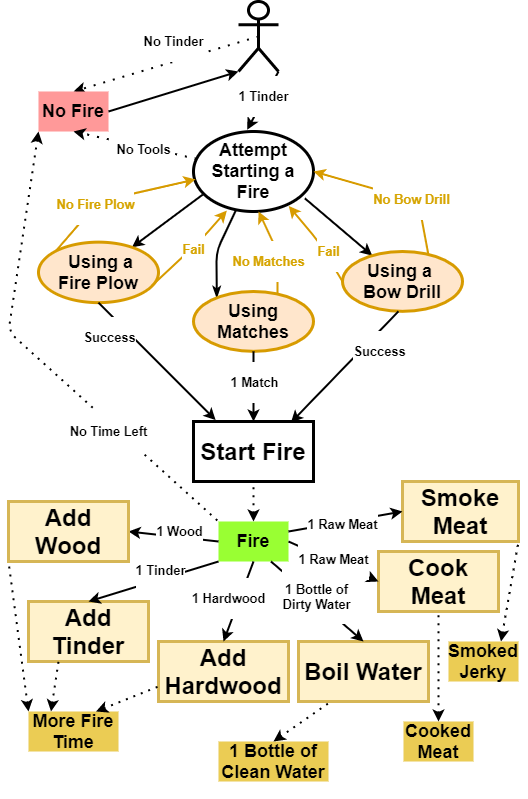
\includegraphics[width=15cm, height=17cm, keepaspectratio]{Images/FireUseCase.png}\\
			\caption{\textbf{Fire Screen Process}}
		\end{figure}


\section{Crafting}
		\par Creating \textbf{complex} items is displayed as \textbf{crafting}, while \textbf{breaking} them apart to get \textbf{parts} can be done in the \textbf{inventory}. Making something new takes \textbf{time} and \textbf{place} near the \textbf{fire}, so it can be done at \textbf{night} with no \textbf{Body Heat loss}.
		\par The \textbf{table} below(\textit{Table 2.10}) showcases all the \textbf{items} that can be \textbf{created}, the \textbf{time} needed, the \textbf{resources} and their \textbf{descriptions}. There can \textbf{only} be \textbf{one} of a certain device in the \textbf{inventory}(Fire Plow, Bow Drill).
		\par \textbf{Crafting} can help with \textbf{Inventory Management} in many ways. There are \textbf{bags} for \textbf{extra space}(Pouch) or \textbf{creations} that are \textbf{more compact} than their \textbf{loose parts}(Wood Bundle, Rope).

		\begin{longtable}{|C{6em}|C{6em}|C{8em}|C{17em}|}
		   \toprule
		   \rowcolor[rgb]{ .647,  .647,  .647} \textcolor[rgb]{ 1,  1,  1}{\textbf{Item}} & \textcolor[rgb]{ 1,  1,  1}{\textbf{Crafting Duration}} & \textcolor[rgb]{ 1,  1,  1}{\textbf{Crafting Resources}} & \textcolor[rgb]{ 1,  1,  1}{\textbf{Description}} \\
		    \midrule
		    \rowcolor[rgb]{ .859,  .859,  .859} \textbf{Fire Plow} & \textbf{30 minutes} & \textbf{Wood} & \textbf{"A primitive tool for starting a fire. Rubbing two sticks together should produce an ember. I can only have one."} \\
		    \midrule
		    \rowcolor[rgb]{ .929,  .929,  .929} \textbf{Bow Drill} & \textbf{30 minutes} & \textbf{Rope, Hardwood} & \textbf{"A primitive tool for starting a fire. Using the bow drill requires some skill and plenty of patience. I can only have one."} \\
		    \midrule
		    \rowcolor[rgb]{ .859,  .859,  .859} \textbf{Fishing Rod} & \textbf{30 minutes} & \textbf{2 Ropes, Fishing Hook, Wood} & \textbf{"A survival fishing rod made of stick, rope, and a hook. Good enough to catch a fish. I can only have one."} \\
		    \midrule
		    \rowcolor[rgb]{ .929,  .929,  .929} \textbf{Wooden Fishing Hook} & \textbf{60 minutes} & \textbf{Wood} & \textbf{"A fishing hook. Sharp end."} \\
		    \midrule
		    \rowcolor[rgb]{ .859,  .859,  .859} \textbf{Rope} & \textbf{30 minutes} & \textbf{Piece Of Cloth} & \textbf{"Piece of rope. Useful for many purposes in a survival situation. Each piece of rope requires 1/3 unit of carry space."} \\
		    \midrule
		    \rowcolor[rgb]{ .929,  .929,  .929} \textbf{Wooden Spear} & \textbf{30 minutes} & \textbf{Hardwood} & \textbf{"It's a wooden spear with a pretty sharp tip. Better than bare handed hunting. I can only have one."} \\
		    \midrule
		    \rowcolor[rgb]{ .859,  .859,  .859} \textbf{Rope Net Bag} & \textbf{180 minutes} & \textbf{3 Ropes} & \textbf{"A survival net bag made of rope. Useful for carrying additional gear[+4 CARRY SPACE]. I can only have one."} \\
		    \midrule
		    \rowcolor[rgb]{ .929,  .929,  .929} \textbf{Pouch} & \textbf{120 minutes} & \textbf{Hare Skin, Rope} & \textbf{"A small pouch. I can carry stuff in it. I can have a couple of these.[+1 CARRY SPACE]"} \\
		    \midrule
		    \rowcolor[rgb]{ .859,  .859,  .859} \textbf{Wood Bundle} & \textbf{60 minutes} & \textbf{4 Woods, Rope} & \textbf{"Bunch of wood tied together. Makes it easier to carry."} \\
   		    \bottomrule	
		\caption{\textbf{Craftable Items}}
		\end{longtable}

	\section{Location Specific Actions}
		\subsection{Exploring}
			\par \textbf{Each time} the player arrives \textbf{somewhere new}, the game takes the \textbf{location type} and uses its \textbf{"Number of Resources"} interval(\textit{Table 2.11}) to \textbf{randomize} how many resources to \textbf{create}.
			\begin{longtable}{|C{7em}|C{4.3em}|C{4.3em}|C{4.3em}|C{4.3em}|C{3.7em}|C{5em}|}
			   \toprule
			   \rowcolor[rgb]{ .647,  .647,  .647} \textcolor[rgb]{ 1,  1,  1}{\textbf{Location}} & \cellcolor[rgb]{ .859,  .859,  .859}\textbf{Pike Lake} & \cellcolor[rgb]{ .859,  .859,  .859}\textbf{Flooded Area} & \cellcolor[rgb]{ .859,  .859,  .859}\textbf{Muddy Road} & \cellcolor[rgb]{ .859,  .859,  .859}\textbf{Muddy Area} & \cellcolor[rgb]{ .859,  .859,  .859}\textbf{Path} & \cellcolor[rgb]{ .859,  .859,  .859}\textbf{Woodland} \\
			   \midrule
			   \rowcolor[rgb]{ .647,  .647,  .647} \textcolor[rgb]{ 1,  1,  1}{\textbf{Number Of Resources}} & \cellcolor[rgb]{ .859,  .859,  .859}\textbf{\{3, 6\}} & \cellcolor[rgb]{ .859,  .859,  .859}\textbf{\{3, 6\}} & \cellcolor[rgb]{ .859,  .859,  .859}\textbf{\{9, 11\}} & \cellcolor[rgb]{ .859,  .859,  .859}\textbf{\{7, 9\}} & \cellcolor[rgb]{ .859,  .859,  .859}\textbf{\{8, 10\}} & \cellcolor[rgb]{ .859,  .859,  .859}\textbf{\{6, 8\}} \\
			   \bottomrule	
			\caption{\textbf{Amount} of \textbf{Resources} at a \textbf{Location Type}}
			\end{longtable}

			\par Each \textbf{location type} has some \textbf{items} and their \textbf{probability to be randomized} in the \textbf{current} place's \textbf{"Available Explorables"} list(\textit{Table 2.12}).
		        \begin{longtable}{|C{10em}|C{4.5em}|C{4.5em}|C{4.5em}|C{3.5em}|C{5em}}
			    \toprule
			    \rowcolor[rgb]{ .647,  .647,  .647} \textcolor[rgb]{ 1,  1,  1}{\textbf{Resource/Location}} & \textcolor[rgb]{ 1,  1,  1}{\textbf{Flooded Area}} & \textcolor[rgb]{ 1,  1,  1}{\textbf{Muddy Road}} & \textcolor[rgb]{ 1,  1,  1}{\textbf{Muddy Area}} & \textcolor[rgb]{ 1,  1,  1}{\textbf{Path}} & \textcolor[rgb]{ 1,  1,  1}{\textbf{Woodland}} \\
			    \midrule
			    \rowcolor[rgb]{ .859,  .859,  .859} \textbf{Wood} & \textbf{-} & \textbf{20\%} & \textbf{35\%} & \textbf{-} & \textbf{-} \\
			    \midrule
			    \rowcolor[rgb]{ .929,  .929,  .929} \textbf{Cattail Plant} & \textbf{-} & \textbf{-} & \textbf{-} & \textbf{24\%} & \textbf{28\%} \\
			    \midrule
			    \rowcolor[rgb]{ .859,  .859,  .859} \textbf{Maggots} & \textbf{17\%} & \textbf{-} & \textbf{-} & \textbf{29\%} &\textbf{38\%} \\
			    \midrule
			    \rowcolor[rgb]{ .929,  .929,  .929} \textbf{Crickets} & \textbf{} & \textbf{14\%} & \textbf{23\%} & \textbf{33\%} &\textbf{28\%} \\
			    \midrule
			    \rowcolor[rgb]{ .859,  .859,  .859} \textbf{Cattail Plant} & \textbf{45\%} & \textbf{-} &\textbf{-} & \textbf{-} & \textbf{-} \\
			    \midrule
			    \rowcolor[rgb]{ .929,  .929,  .929} \textbf{Edible Berries} & \textbf{-} & \textbf{22\%} & \textbf{12\%} & \textbf{14\%} & \textbf{6\%} \\
			    \midrule
			    \rowcolor[rgb]{ .859,  .859,  .859} \textbf{Plant Fiber} & \textbf{38\%} & \textbf{9\%} & \textbf{23\%} & \textbf{-} & \textbf{-} \\
			    \midrule
			    \rowcolor[rgb]{ .929,  .929,  .929} \textbf{Birch Bark} & \textbf{-} & \textbf{24\%} & \textbf{7\%} & \textbf{-} & \textbf{-} \\
			    \bottomrule	
			\caption{\textbf{Chance} of \textbf{Item} \textbf{Finding} at Certain \textbf{Locations}}
			\end{longtable}

			\par \textbf{Pike Lake} has some \textbf{exclusive} items that are \textbf{very useful} for the \textbf{gameplay}, as it can only be visited \textbf{once}, at the beginning.(\textit{Table 2.13}).

			\begin{longtable}{|C{2.4em}|C{3.2em}|C{3.0em}|C{3.2em}|C{3.4em}|C{2.8em}|C{3.5em}|C{4.0em}|C{4.0em}|}
			    \toprule
			    \rowcolor[rgb]{ .647,  .647,  .647} \textcolor[rgb]{ 1,  1,  1}{\textbf{Item}} & \cellcolor[rgb]{ .859,  .859,  .859}\textbf{Flash Light} & \cellcolor[rgb]{ .859,  .859,  .859}\textbf{Wires} & \cellcolor[rgb]{ .859,  .859,  .859}\textbf{Empty Bottle} & \cellcolor[rgb]{ .859,  .859,  .859}\textbf{News Paper} & \cellcolor[rgb]{ .859,  .859,  .859}\textbf{Duct Tape} & \cellcolor[rgb]{ .859,  .859,  .859}\textbf{Fishing Kit} & \cellcolor[rgb]{ .859,  .859,  .859}\textbf{Matches} & \cellcolor[rgb]{ .859,  .859,  .859}\textbf{First Aid Kit} \\
			    \midrule
			    \rowcolor[rgb]{ .647,  .647,  .647} \textcolor[rgb]{ 1,  1,  1}{\textbf{\%}} & \cellcolor[rgb]{ .929,  .929,  .929}\textbf{15\%} & \cellcolor[rgb]{ .929,  .929,  .929}\textbf{25\%} & \cellcolor[rgb]{ .929,  .929,  .929}\textbf{10\%} & \cellcolor[rgb]{ .929,  .929,  .929}\textbf{15\%} & \cellcolor[rgb]{ .929,  .929,  .929}\textbf{9\%} & \cellcolor[rgb]{ .929,  .929,  .929}\textbf{8\%} & \cellcolor[rgb]{ .929,  .929,  .929}\textbf{8\%} & \cellcolor[rgb]{ .929,  .929,  .929}\textbf{10\%} \\
			     \bottomrule	
			\caption{\textbf{Chance} of \textbf{Finding} an \textbf{Item} at \textbf{Pike Lake}}
			\end{longtable}

		\subsection{Getting Wood}
		\par \textbf{Wood} can't be collected at \textbf{Pike Lake}, in order to promote \textbf{Exploring} for \textbf{new players} and because the \textbf{car} acts as a \textbf{shelter}. There is \textbf{no limit} at any locations, the player only has the \textbf{night} without a \textbf{flaslight} to worry about.

		\subsection{Getting Water}
			\par \textbf{Clean water} can be obtained through a \textbf{raincatcher}, but \textbf{dirty water} can be collected from locations that have it as a \textbf{resource}(\textit{Table 2.14}).
			\begin{longtable}{|C{7em}|C{3.5em}|C{4.5em}|C{4.5em}|C{4.5em}|C{3.5em}|C{5em}|}
			   \toprule
			   \rowcolor[rgb]{ .647,  .647,  .647} \textcolor[rgb]{ 1,  1,  1}{\textbf{Location}} & \cellcolor[rgb]{ .859,  .859,  .859}\textbf{Pike Lake} & \cellcolor[rgb]{ .859,  .859,  .859}\textbf{Flooded Area} & \cellcolor[rgb]{ .859,  .859,  .859}\textbf{Muddy Road} & \cellcolor[rgb]{ .859,  .859,  .859}\textbf{Muddy Area} & \cellcolor[rgb]{ .859,  .859,  .859}\textbf{Path} & \cellcolor[rgb]{ .859,  .859,  .859}\textbf{Woodland} \\
			  \midrule			    
			  \rowcolor[rgb]{ .647,  .647,  .647} \textcolor[rgb]{ 1,  1,  1}{\textbf{Dirty Water Source}} & \cellcolor[rgb]{ .859,  .859,  .859}\textbf{Yes} & \cellcolor[rgb]{ .859,  .859,  .859}\textbf{Yes} & \cellcolor[rgb]{ .859,  .859,  .859}\textbf{No} & \cellcolor[rgb]{ .859,  .859,  .859}\textbf{Yes} & \cellcolor[rgb]{ .859,  .859,  .859}\textbf{No} & \cellcolor[rgb]{ .859,  .859,  .859}\textbf{No} \\
			    \bottomrule	
			\caption{\textbf{Location Types} \textbf{Water Resources}}
			\end{longtable}
		
		\subsection{Setting Traps and Catching Fish}
		
		\par \textbf{Traps} have their own \textbf{screen} that allows \textbf{building and dismantling}. The \textbf{amount} that can be made of each is  \textbf{infinite} if the resources are there, so the  \textbf{chance} gets \textbf{better} with each  \textbf{new one}(\textit{Table 2.15}). \textbf{Fish} can be caught with a \textbf{spear}(5\%) or \textbf{fished}(8\%).
			\begin{longtable}{|C{6em}|C{6em}|C{5em}|C{9em}|C{9em}|}
			   \toprule
			   \rowcolor[rgb]{ .647,  .647,  .647} \textcolor[rgb]{ 1,  1,  1}{\textbf{Traps}} & \textcolor[rgb]{ 1,  1,  1}{\textbf{Hourly Trap Rate}} & \textcolor[rgb]{ 1,  1,  1}{\textbf{Prey}} & \textcolor[rgb]{ 1,  1,  1}{\textbf{Prey Resources}} & \textcolor[rgb]{ 1,  1,  1}{\textbf{Building Resources}} \\
			    \midrule
			    \rowcolor[rgb]{ .859,  .859,  .859} \textbf{Deadfall} & \textbf{2\%} & \textbf{Hare} & \textbf{3 Raw Meats, Bait, Hare Skin} & \textbf{Rope, Wood, Bait} \\
			    \midrule
			    \rowcolor[rgb]{ .929,  .929,  .929} \textbf{Fish Trap} & \textbf{3\%} & \textbf{Fish} & \textbf{1 Raw Meat} & \textbf{Rope, Wood, Bait} \\
			    \midrule
			    \rowcolor[rgb]{ .859,  .859,  .859} \textbf{Bird Trap} & \textbf{4\%} & \textbf{Bird} & \textbf{2 Raw Meats} & \textbf{Rope, Wood, Bait} \\
			    \bottomrule
			\caption{\textbf{Traps} }	
			\end{longtable}

	\section{Travel}
		\par \textbf{Travelling} to a location requires an \textbf{inventory} below the \textbf{space threshold}. The \textbf{number} of travel hours is \textbf{randomized} from the specific \textbf{interval}. 
		\par If the player has less than \underline{400} calories, \underline{2} \textbf{extra hours} are added to the \textbf{trip}. The location \textbf{choices} are \textbf{not visible} at night without a \textbf{flashlight}(\textit{Table 2.16}).
		\begin{longtable}{|C{10.555em}|C{5.22em}|C{5.22em}|C{6.445em}|}
		    \toprule			    
		    \rowcolor[rgb]{ .647,  .647,  .647} \textcolor[rgb]{ 1,  1,  1}{\textbf{Location}} & \textcolor[rgb]{ 1,  1,  1}{\textbf{Miles}} & \textcolor[rgb]{ 1,  1,  1}{\textbf{Hours}} & \textcolor[rgb]{ 1,  1,  1}{\textbf{Water Source}} \\
		    \midrule
		    \rowcolor[rgb]{ .859,  .859,  .859} \textbf{Pike Lake} & \textbf{3} & \textbf{\{4, 5\}} & \textbf{Yes} \\
		    \midrule
		    \rowcolor[rgb]{ .929,  .929,  .929} \textbf{Flooded Area} & \textbf{2} & \textbf{\{4, 5\}} & \textbf{Yes} \\
		    \midrule
		    \rowcolor[rgb]{ .859,  .859,  .859} \textbf{Muddy Road} & \textbf{2} & \textbf{\{3, 4\}} & \textbf{No} \\
		    \midrule
		    \rowcolor[rgb]{ .929,  .929,  .929} \textbf{Muddy Area} & \textbf{2} & \textbf{\{3, 4\}} & \textbf{Yes} \\
		    \midrule
		    \rowcolor[rgb]{ .859,  .859,  .859} \textbf{Path} & \textbf{3} & \textbf{\{3, 4\}} & \textbf{No} \\
		    \midrule
		    \rowcolor[rgb]{ .929,  .929,  .929} \textbf{Woodland} & \textbf{2} & \textbf{\{3, 4\}} & \textbf{No} \\
		    \bottomrule
		\caption{\textbf{Travel Information} }	
		\end{longtable}


\newpage

\chapter{Implementation} 

	\section{Technologies}
		\subsection{Kivy}
			\par \textbf{Kivy}\cite{Kivy} is a \textbf{cross-platform framework} that allowed me to build the game as an \textbf{Android application}. The \textbf{relationship} between \textbf{Kivy} and \textbf{Python} reminds me heavily of the one between \textbf{CSS/HTML} and \textbf{PHP}. Placing \textbf{Widgets} in \underline{".kv"} files feels like building a \textbf{web site}. My \textbf{text-based, screen-heavy} game took \textbf{thousands} of lines of \textbf{Kivy} code. 

		\subsection{Pickle}
			\par \textbf{Pickle}\cite{Pickle} is a \textbf{Python} module used for \textbf{serializing object structures}. I used it to implement \textbf{saving, loading} and \textbf{pausing} on a \textbf{Game State object} that holds all the \textbf{information} about the \textbf{gameplay}. 
		
	\subsection{Buildozer}
		\par \textbf{Buildozer}\cite{Buildozer} is a tool that packages \textbf{mobile} applications. I used it to create the \textbf{Android executable} for the game. It requires \textbf{Linux} for compilation, so I shared the code between \textbf{Ubuntu} and \textbf{Windows} via \textbf{Github} in order to use it.
	
	\section{Integration}
		\begin{figure}[H]
			\centering
			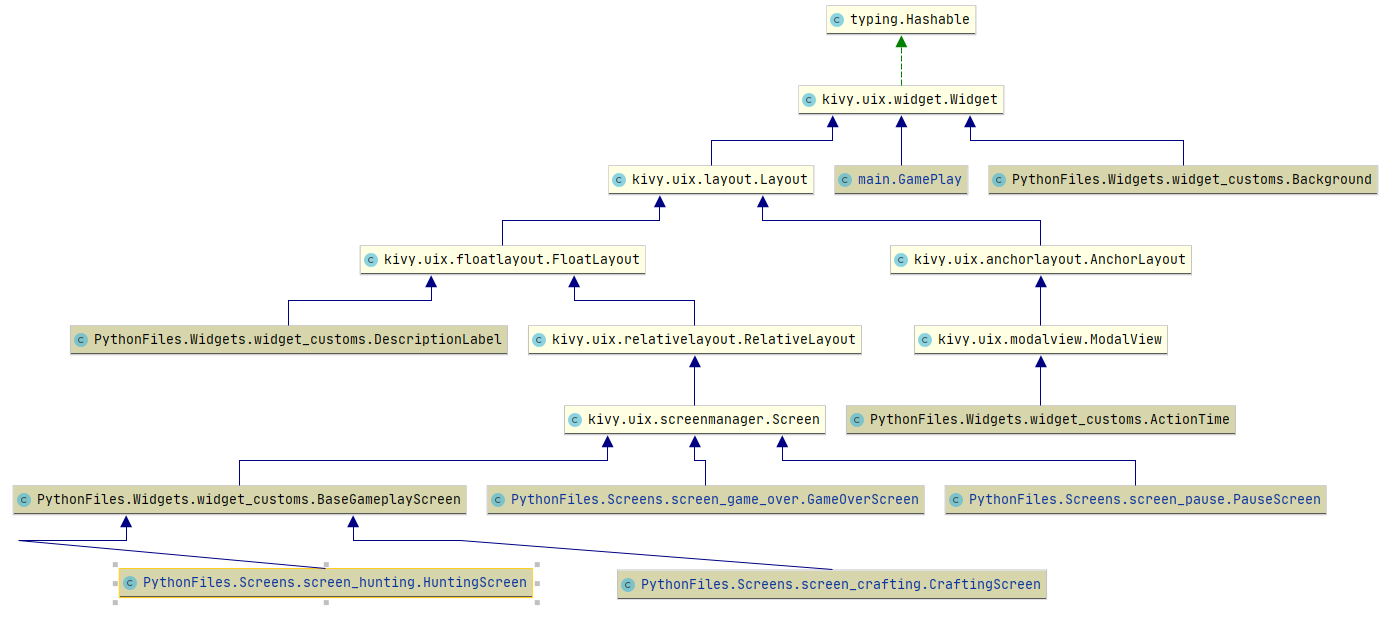
\includegraphics[width=14cm, height=9cm, keepaspectratio]{Images/Diagram.png}\\
			\caption{\textbf{Piece of Kivy and Python Integration Architecture}}
		\end{figure}
		\par \textbf{Python} makes use of \textbf{Kivy Widgets} in order to create \textbf{UI elements}. This can be seen in \textit{Figure 3.1}, which contains a piece of \textbf{integration architecture}(with most elements discarded to fit).
	
		\subsection{Kivy Using Kivy Files}
			\par \textbf{Kivy} code can be written in both \underline{".kv"} and \underline{".py"} files. \textit{Listing 3.1} displays a piece of code that adds a \textbf{Button Widget} and an \textbf{Image Widget}(a "pause" symbol) to three selected \textbf{screens}.
			\par The language's \textbf{structure} resembles \textbf{HTML}. It allows for compact code as \textbf{multiple screens} can share the same \textbf{Widgets}. The \underline{"root.show\_info()"} line calls the \underline{"show\_info()"} \textbf{method} of the \textbf{parent object} found in a ".py" file. The \underline{"on\_release"} line allows behaviour addition and makes the button \textbf{responsive}. The \textbf{image} is added on top and does not \textbf{interfere} with the \textbf{functionality} of the \textbf{button}.
			\begin{lstlisting}[caption={\textbf{Kivy} Implementation of the \textbf{Pause Button}},captionpos=b]
<FireScreen, HuntingScreen, ShelterScreen>:
    FloatLayout:
        Button:
            pos_hint:{"x": 0.91, "y": 0.90}
            size_hint: 0.04, 0.07
            background_color: 0.0, 0.0, 0.0, 1.0
            bold: True
            font_size: self.height*0.5
            text: ""
            on_release:
                root.show_info()
        Image:
            source: "GraphicFiles/info.png"
            size_hint: 0.026, 0.054
            pos_hint:{"x": 0.917, "y": 0.908}
            allow_stretch: True
			\end{lstlisting}

		\subsection{Kivy Using Python Files}
		\par \textbf{Widgets} can be \textbf{implemented} in \underline{".py"} files as well. \textbf{"ModalView"} creates a \textbf{Pop Up} the size of the current window. The code in \textit{Listing 3.2} implements a \textbf{"ModalView"} that displays an \textbf{"action execution"} text and \textbf{closes} after a second("Building...", "Sleeping...").
			\begin{lstlisting}[caption={\textbf{Kivy} Implementation of the\textbf{Action Execution Pop Up}},captionpos=b]
class ActionTime(ModalView):

    def __init__(self, text, **kwargs):
        super(ActionTime, self).__init__(**kwargs)

        # Set the specific text for the action
        self.ids.action_time_label.text = text

        # Call dismiss_view after one second
        Clock.schedule_once(self.dismiss_view, 1)

    def dismiss_view(self, dt):
        self.dismiss()
			\end{lstlisting}
	
			\par \textit{Listing 3.3} \textbf{showcases} the piece of code that \textbf{changes} the \textbf{background} picture to reflect the \textbf{time} of the day.
			
\begin{lstlisting}[caption={\textbf{Kivy} Implementation of the \textbf{Background Change}},captionpos=b]
class Background(Widget):
    """ Class for changing the background during the day """

    # The path to background image
    this_source = StringProperty("GraphicFiles/night.png")

    def change_background(self, *args):
        """ Change background after the day period """
        # Total game hours that have passed
        game_hours = init.game_state.game_time / 60
        # The current day of the game
        init.game_state.current_game_day = int(game_hours / 24 + 1)
        # Game hours that have passed in the current day
        game_hours_today = game_hours % 24

        # Change background image path based on the time of the day
        if game_hours_today < 2:
            self.this_source = "GraphicFiles/dawn.png"
        if game_hours_today < 7:
            self.this_source = "GraphicFiles/orange.png"
        elif game_hours_today < 10:
            self.this_source = "GraphicFiles/purple.png"
        elif game_hours_today < 12:
            self.this_source = "GraphicFiles/sunset.png"
        else:
            self.this_source = "GraphicFiles/night.png"
			\end{lstlisting}

	\section{Testing} 
		\par The \textbf{project} was \textbf{manually} tested after each \textbf{iteration}. The nature of the game allows for extremely \textbf{fast playthroughs}, as each action takes \textbf{one second} in real time. This was a \textbf{best case} scenario, as each feature could be \textbf{tested} in a matter of at most \textbf{several minutes}. Testing \textbf{automation} was not really needed.
		
		\subsection{Quality Assurance}
			\par As far as I am concerned, there are \textbf{no bugs} remaining. The addition of the \textbf{rain} \underline{".gif"} \textbf{animation} makes the \textbf{game} take a minute to \textbf{open} on \textbf{mobile devices} after the first installation, but the application is very \textbf{responsive} otherwise. \textbf{"Speedruns"} can cause \textbf{occasional} lags of 2-3 seconds, but \textbf{fast gameplay} poses no problems.

		\subsection{Playtesting}
			\par The \textbf{application} was \textbf{tested} by friends, family and other students. As I was implementing an already \textbf{successful game}, I didn't really have many \textbf{difficulties} with the \textbf{mechanics} and \textbf{gameplay design} choices. However, there are things that I \textbf{changed} to \textbf{my liking} and I made sure to \textbf{cater} to all the \textbf{complaints} and \textbf{suggestions}.
	
\newpage

\chapter*{Conclusion}
\addcontentsline{toc}{chapter}{Conclusion}
	\par Making this \textbf{game} was a very \textbf{gratifying} and \textbf{fulfilling} experience. I succeeded to \textbf{implement} all of the \textbf{mechanics} and \textbf{features} of the original game's \textbf{medium difficulty} gameplay. The application can be \textbf{downloaded} and \textbf{played} on \textbf{Android }mobile devices. 
	\par The \textbf{user} can \textbf{pause, resume, save} and \textbf{quit} the game with no negative impact on the \textbf{time progression} and the \textbf{permanent death} feature. The \textbf{environment} has all the original \textbf{locations} and \textbf{resources}. \textbf{Sleeping, crafting, travel, traps} and \textbf{hunting} were also fully implemented. All the \textbf{inventory items} can be manipulated and used in the intended ways. \textbf{Exploration} and \textbf{resource gathering} have similar, if not identical chance \textbf{values}. 
	\par The \textbf{graphical interface} has \textbf{bright colours} and \textbf{beautiful backgrounds}. The \textbf{screen structure} is similar, but the \textbf{design} was tweaked to my liking. I did not, however, manage to implement a \textbf{sound} system.
	\par I chose to make the \textbf{game} in \textbf{Python} because I have done this before and I was \textbf{comfortable} with it. I am glad I took the time to make a lot of the \textbf{GUI} elements from \textbf{scratch} and learn about \textbf{integration}, but I will not do this again. I cherish the \textbf{knowledge}, but I have gained enough \textbf{confidence} to use \textbf{game engines} from now on.
	\par In \textbf{conclusion}, all of the primary \textbf{objectives} of the \textbf{project} have been \textbf{achieved}.
\newpage

\begin{thebibliography}{99}

\bibitem{Survive}
Survive - Wilderness Survival  \\
{https://play.google.com/store/apps/details?id=com.sandbaygames.survive\&hl=ro\&gl=US}

\bibitem{Juuso}
Juuso Hietalahti \\
\textit{https://fi.linkedin.com/in/juusohietalahti}

\bibitem{Course}
Game Design Course \\
\textit{https://profs.info.uaic.ro/~mmoruz/courses/GD2021.html}

\bibitem{Method}
Iterative Game Design Diagram \\
\textit{http://www.backyardgamedesign.com/blog/2015/5/11/game-design-process}

\bibitem{Pygame}
Pygame Documentation \\
\textit{https://www.pygame.org/news }
 
\bibitem{Kivy}
Kivy Documentation \\
\textit{https://kivy.org/\#home}

\bibitem{Pickle}
Pickle Documentation \\
\textit{https://docs.python.org/3/library/pickle.html}
 
\bibitem{Buildozer}
Buildozer Documentation \\
\textit{https://buildozer.readthedocs.io/en/latest/}

\bibitem{Icon}
Flaticon - Inventory Item Icons \\
\textit{https://www.flaticon.com/search?word=wood}
 
\bibitem{tree}
pngtree - Background Images \\
\textit{https://pngtree.com/user/my-favorites?type=back\&page=2}
 
\end{thebibliography}


\end{document}